\section{Vorgehen Versuch 1}
Nachfolgend haben wir das Vorgehen von unserem ersten Versuch in einer Grafik übersichtlich dargestellt. Die Blitze deuten dabei auf ein Hindernis bei welchem mehr Aufwand benötigt wurde hin und das rote X als einen fehlgeschlagenen Versuch, welcher abgebrochen werden musste.
\begin{figure}[H]
	\centering
	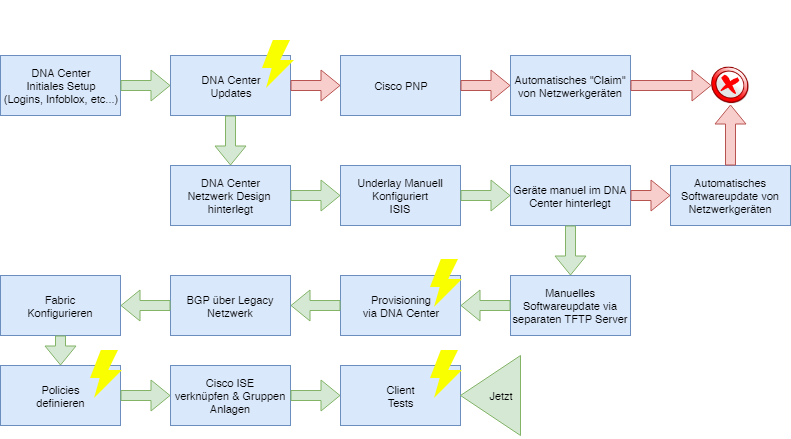
\includegraphics[height=9cm]{img/vorgehen.png}
	\caption{Übersicht Vorgehen}
	\label{fig:vorgehen}
\end{figure} 

\subsection{DNA Center Initiales Setup}

\subsubsection{Installation}
\label{DNACenterSetup_Installation}
Die Installation des DNA Centers erfolgt direkt an der Konsole oder über die Cisco IMC. Dabei wird der maglev-config-wizard ausgeführt. Dieser Befehl kann zu einem späteren Zeitpunkt erneut ausgeführt werden, wenn die Konfiguration angepasst werden muss.

Wie in Kapitel 2\cite{cisco-dna-installation-guide} beschrieben werden folgende Angaben benötigt:
\begin{itemize}
	\item Host IP Adresse
	\item Netmask
	\item Default Gateway IP adress
	\item DNS Servers
	\item Static Routes
	\item HTTPS Proxy
	\item Maglev Master Node IP
	\item Username, Passwort und Linux Passwort
	\item Administration Passphrase für das Web-Interface
	\item NTP Server
	\item Service Subnets
\end{itemize}

Im ersten Schritt \ref{fig:dna-center-install-step-1} wird gewählt, ob ein neuer Cluster erstellt werden soll oder einem beigetreten werden soll. Bei der Testumgebung dieser Arbeit war nur eine Appliance verfügbar, weshalb schliesslich "Start a DNA-C Cluster" ausgewählt wurde. 

\begin{figure}[H]
	\centering
	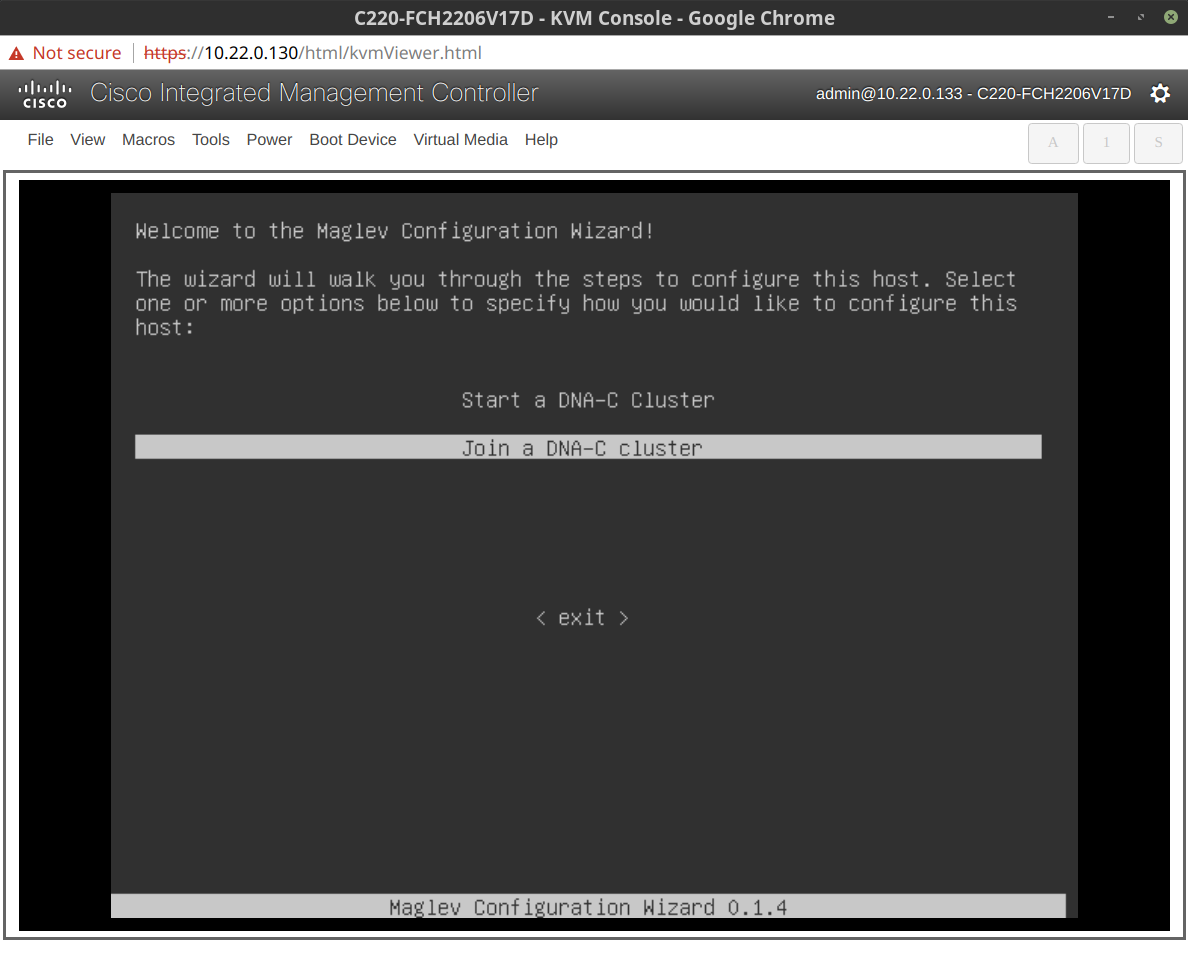
\includegraphics[height=9cm]{img/sc_001.png}
	\caption{DNA Center Configuration Wizard - Start}
	\label{fig:dna-center-install-step-1}
\end{figure} 

Im nächsten Schritt muss die IP Konfiguration für die DNA Center Appliance angegeben werden. Es muss mindestens ein Interface konfiguriert werden und als Cluster Link definiert sein. Statische Routen können definiert werden, sind aber optional.

\begin{figure}[H]
	\centering
	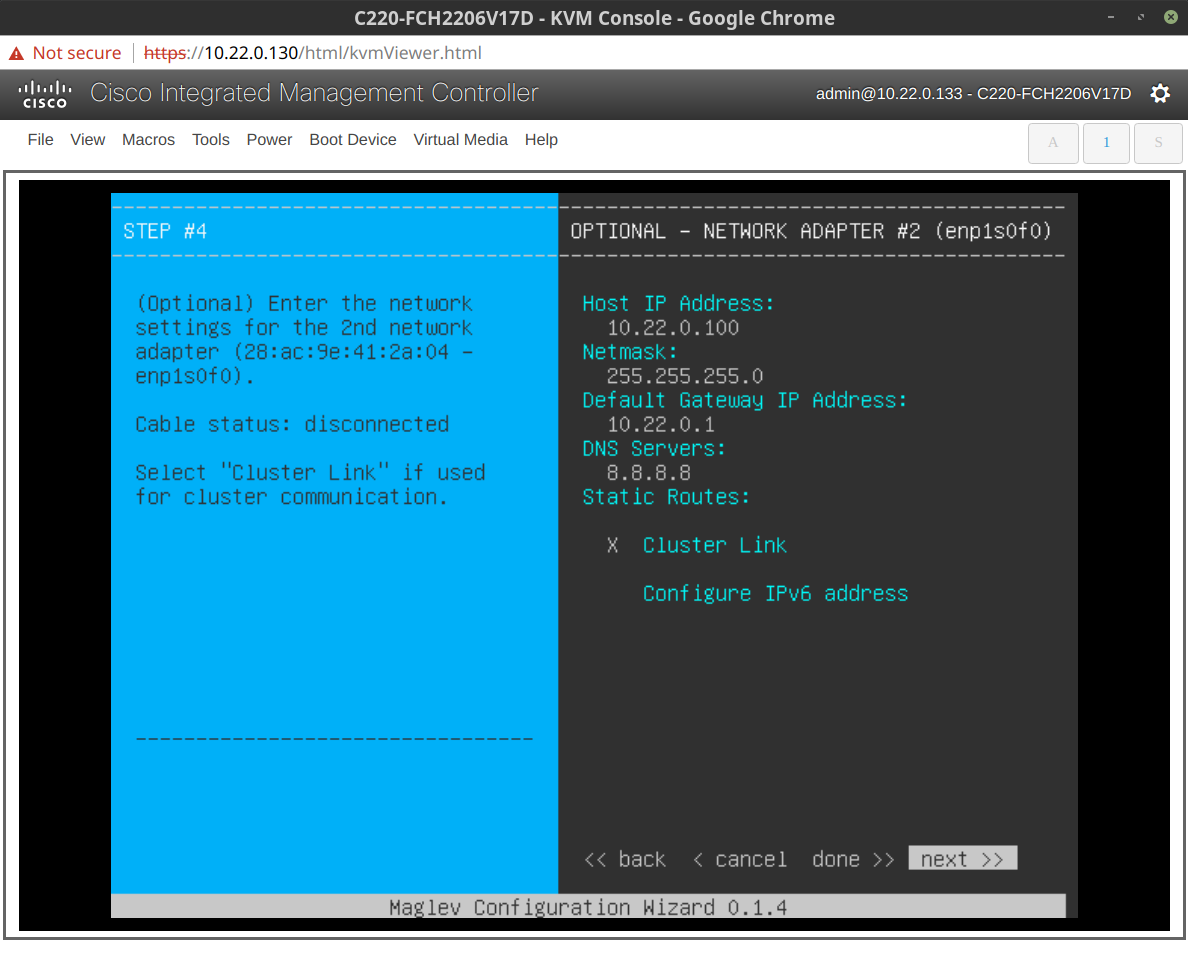
\includegraphics[height=9cm]{img/sc_002.png}
	\caption{DNA Center Configuration Wizard - Entering Management IP}
	\label{fig:dna-center-install-step-4}
\end{figure} 

Im letzten Schritt des Wizards werden alle User Account Einstellungen festgelegt. Hier bei ist zu beachten, dass das "Linux Password" für den SSH Zugriff benötigt wird und die "Administrator Passphrase" für den Zugang zum Web Interface.
 
\begin{figure}[H]
	\centering
	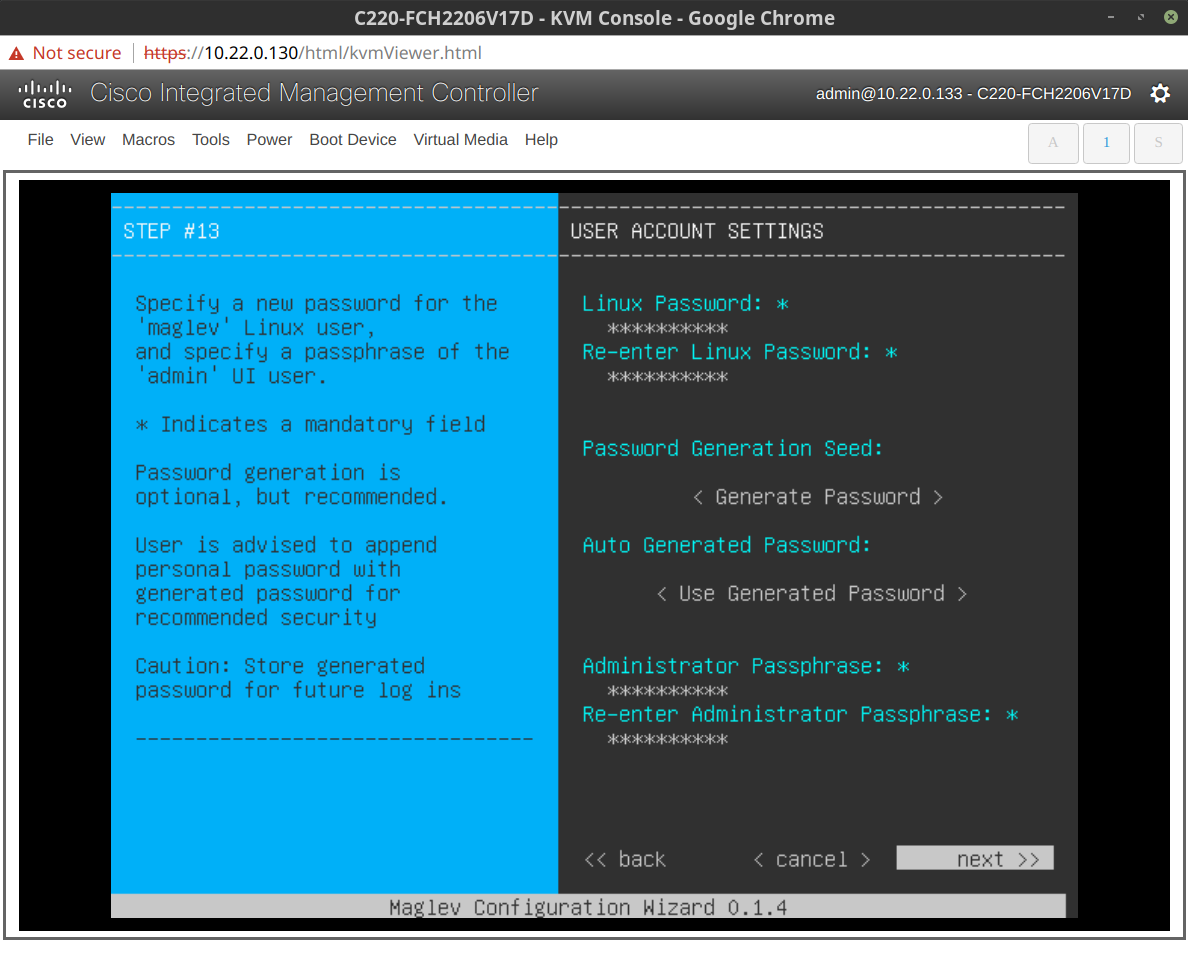
\includegraphics[height=9cm]{img/sc_003.png}
	\caption{DNA Center Configuration Wizard - Entering Authentification Data}
	\label{fig:dna-center-install-step-13}
\end{figure}

Nun wird das DNA Center aufgesetzt. Dieser Prozess dauert mehrere Stunden. 

\begin{figure}[H]
	\centering
	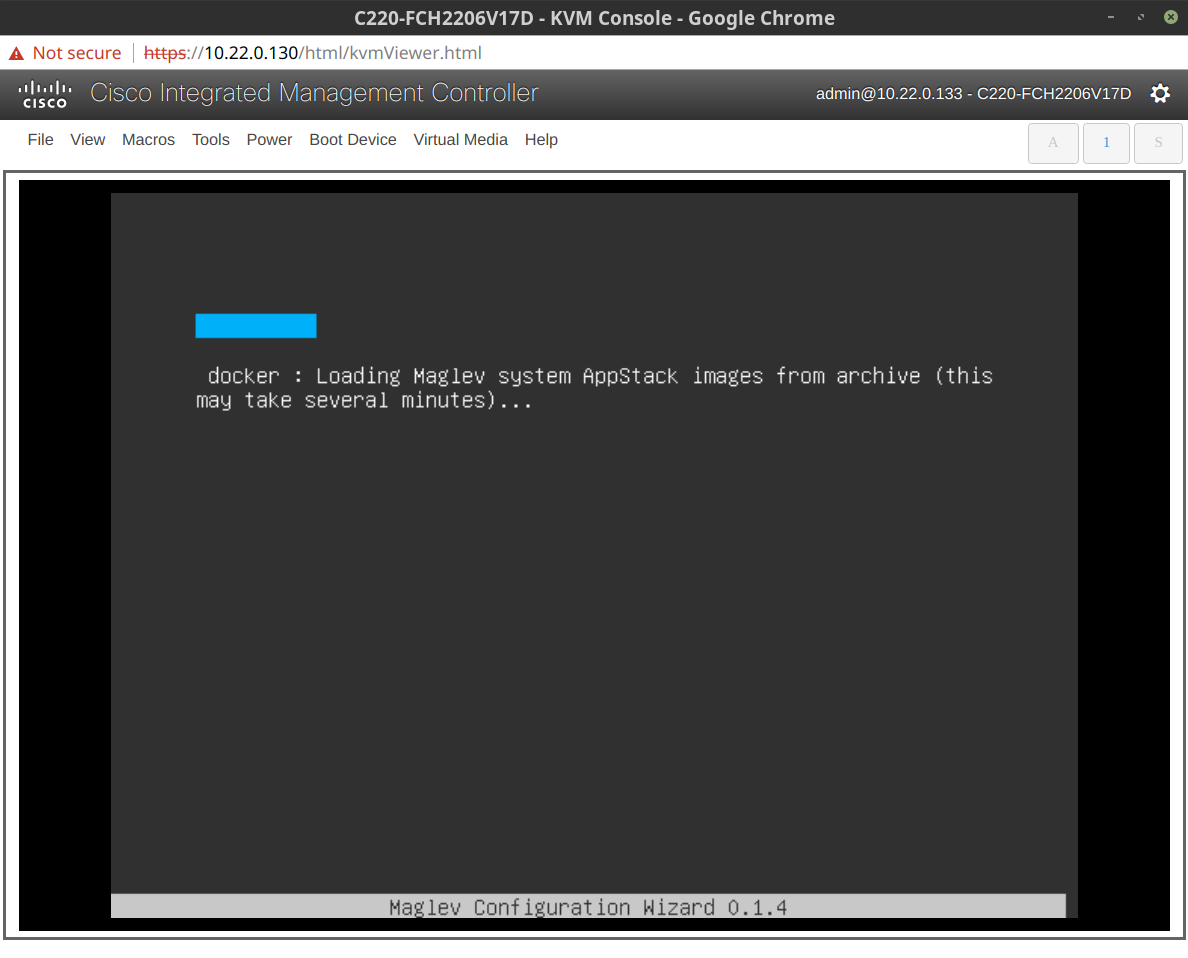
\includegraphics[height=9cm]{img/sc_004.png}
	\caption{DNA Center Configuration Wizard - DNA Center uses docker}
	\label{fig:dna-center-install-step-install}
\end{figure}


\subsubsection{Setup Accounts}
Nach dem der Wizard die Installation vollständig ausgeführt hat, ist das DNA Center Web-GUI verfügbar. Die Konfiguration kann nun über dieses weitergeführt werden.
\begin{figure}[H]
	\centering
	\includegraphics[height=9cm]{img/sc_005.png}
	\caption{DNA Center Web GUI - Login Page}
	\label{fig:dna-center-gui-1}
\end{figure}

Gleich zu Beginn verlangt das DNA Center die Cisco Credentials die mit dem Smart Account verknüpft sind, in welchem die Lizenzen verwaltet werden. Diese Informationen können auch zu einem späteren Zeitpunkt noch eingetragen werden.

\begin{figure}[H]
	\centering
	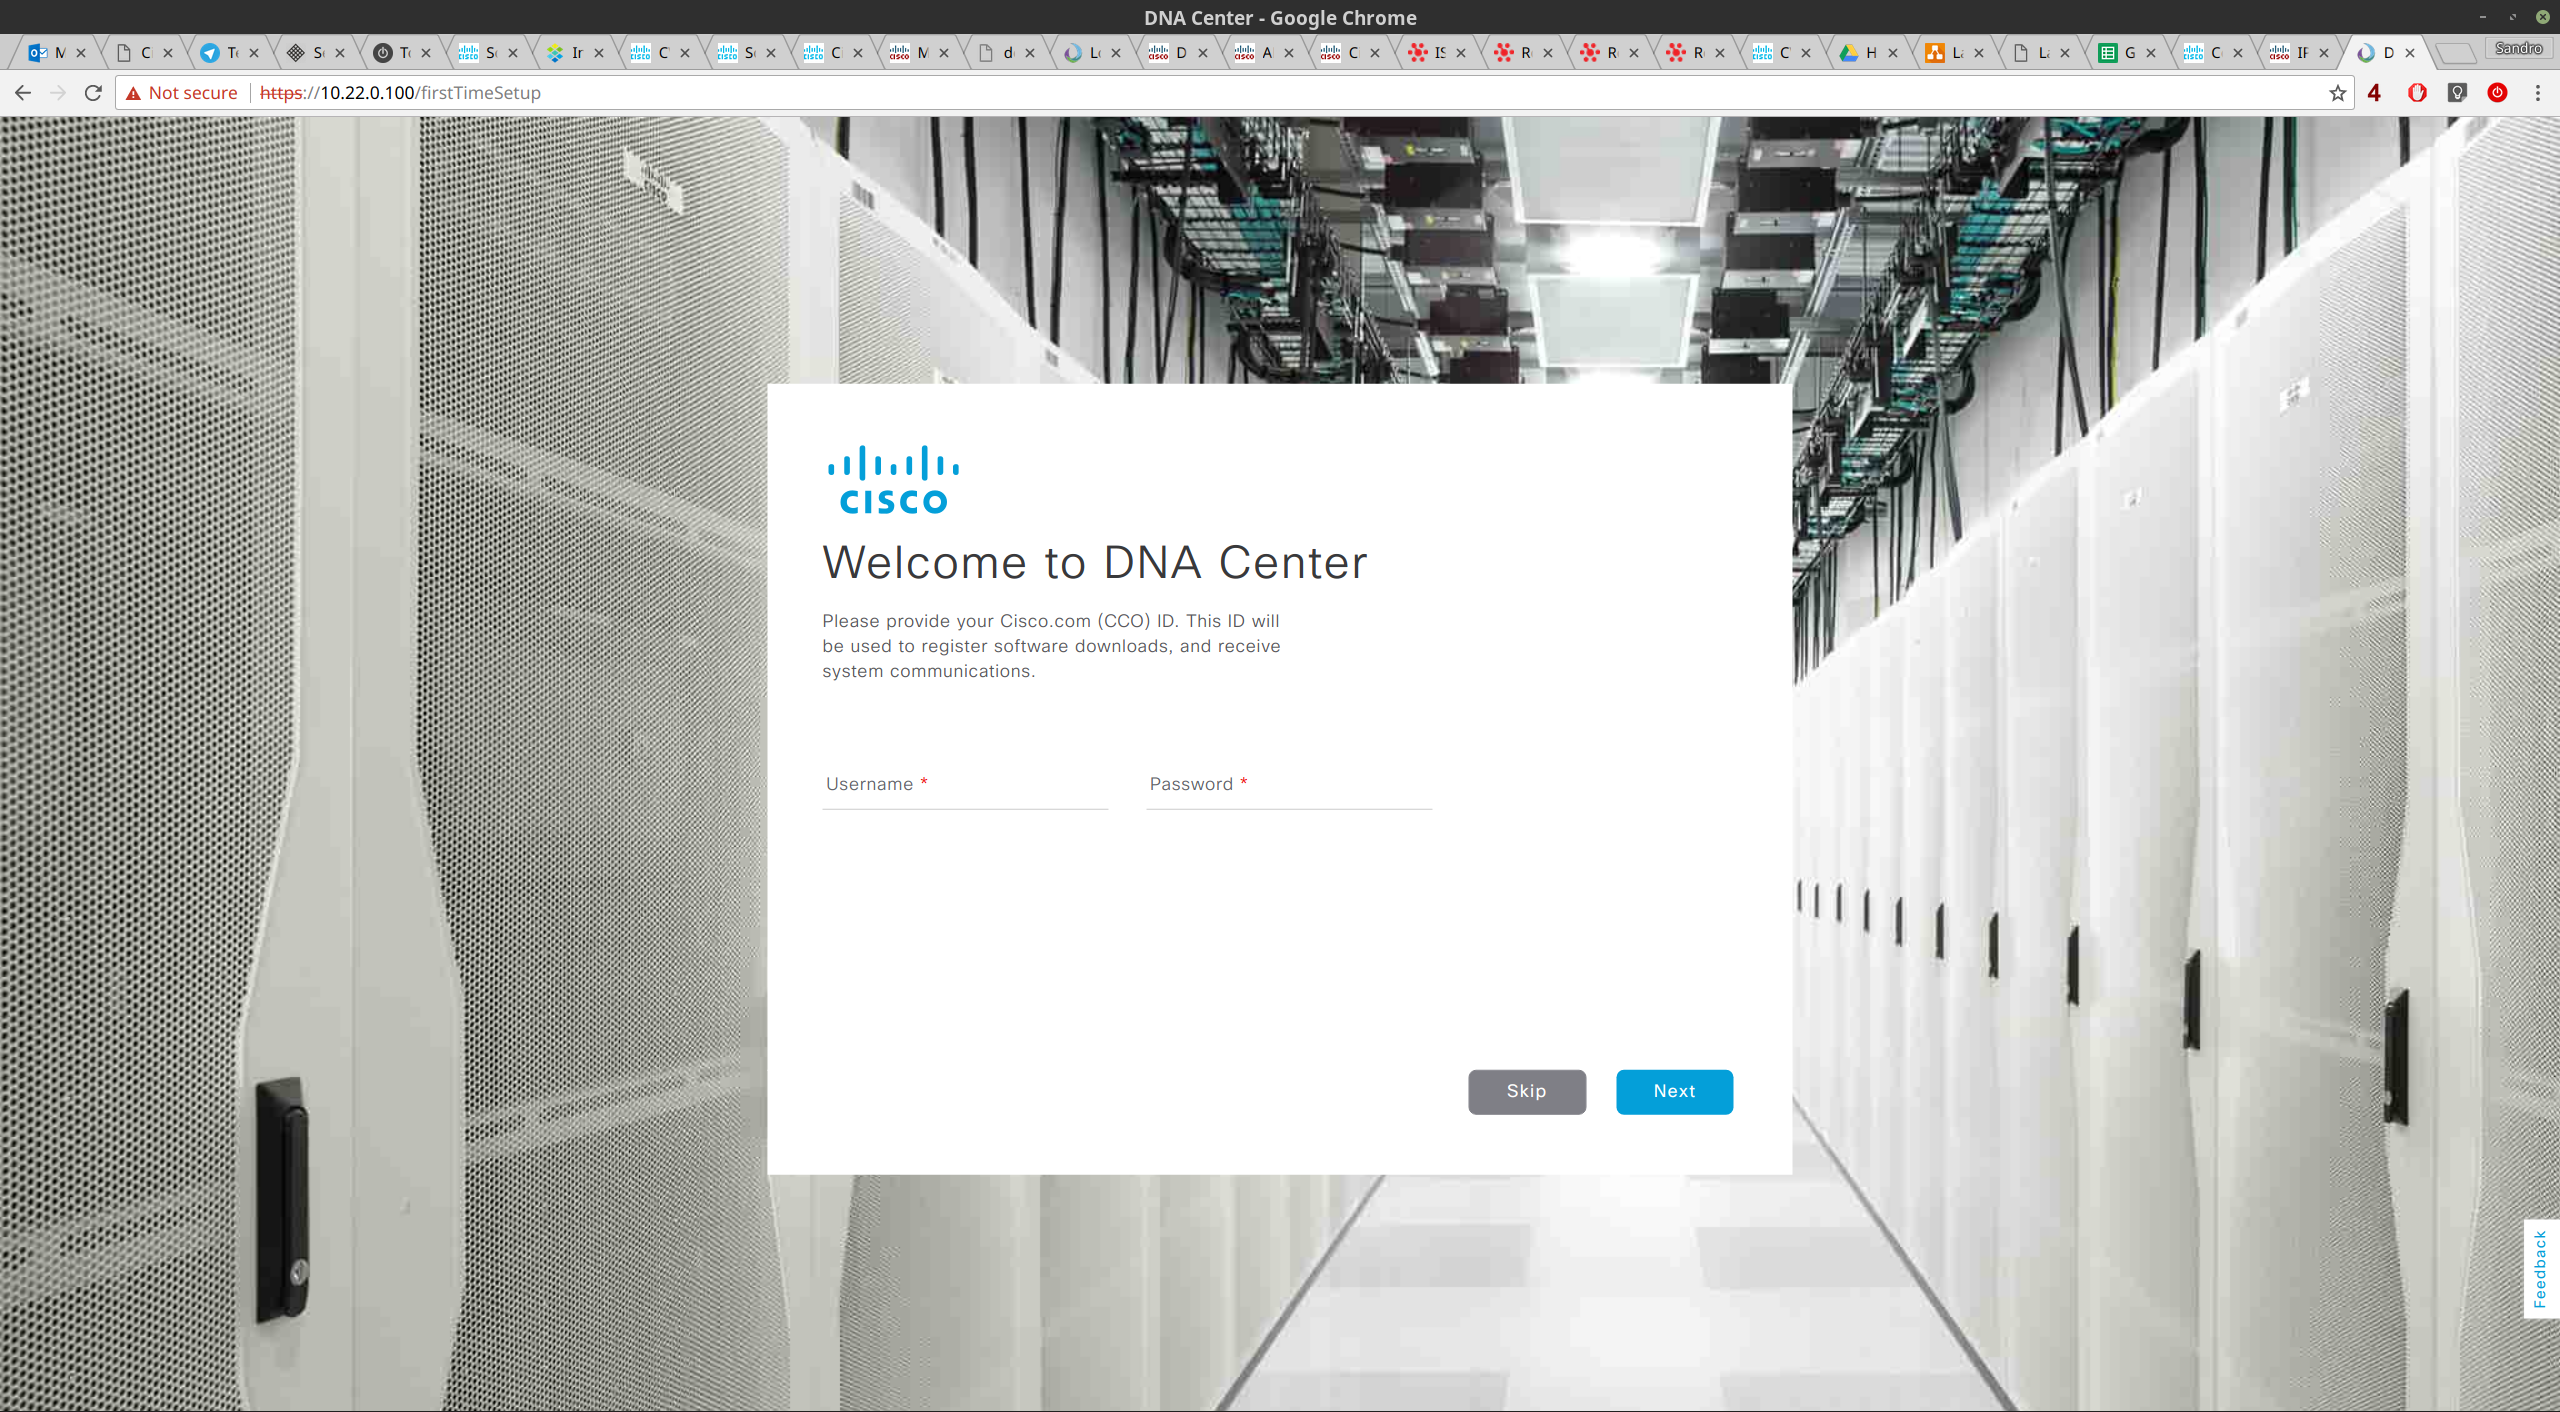
\includegraphics[height=9cm]{img/sc_006.png}
	\caption{DNA Center Web GUI - Cisco Credentials for Licences}
	\label{fig:dna-center-gui-2}
\end{figure}

Im nächsten Schritt kann ein IPAM Server angegeben werden. Diese Einstellung kann ebenfalls später angepasst werden, weshalb wir diesen Schritt zu Beginn übersprungen haben.

\begin{figure}[H]
	\centering
	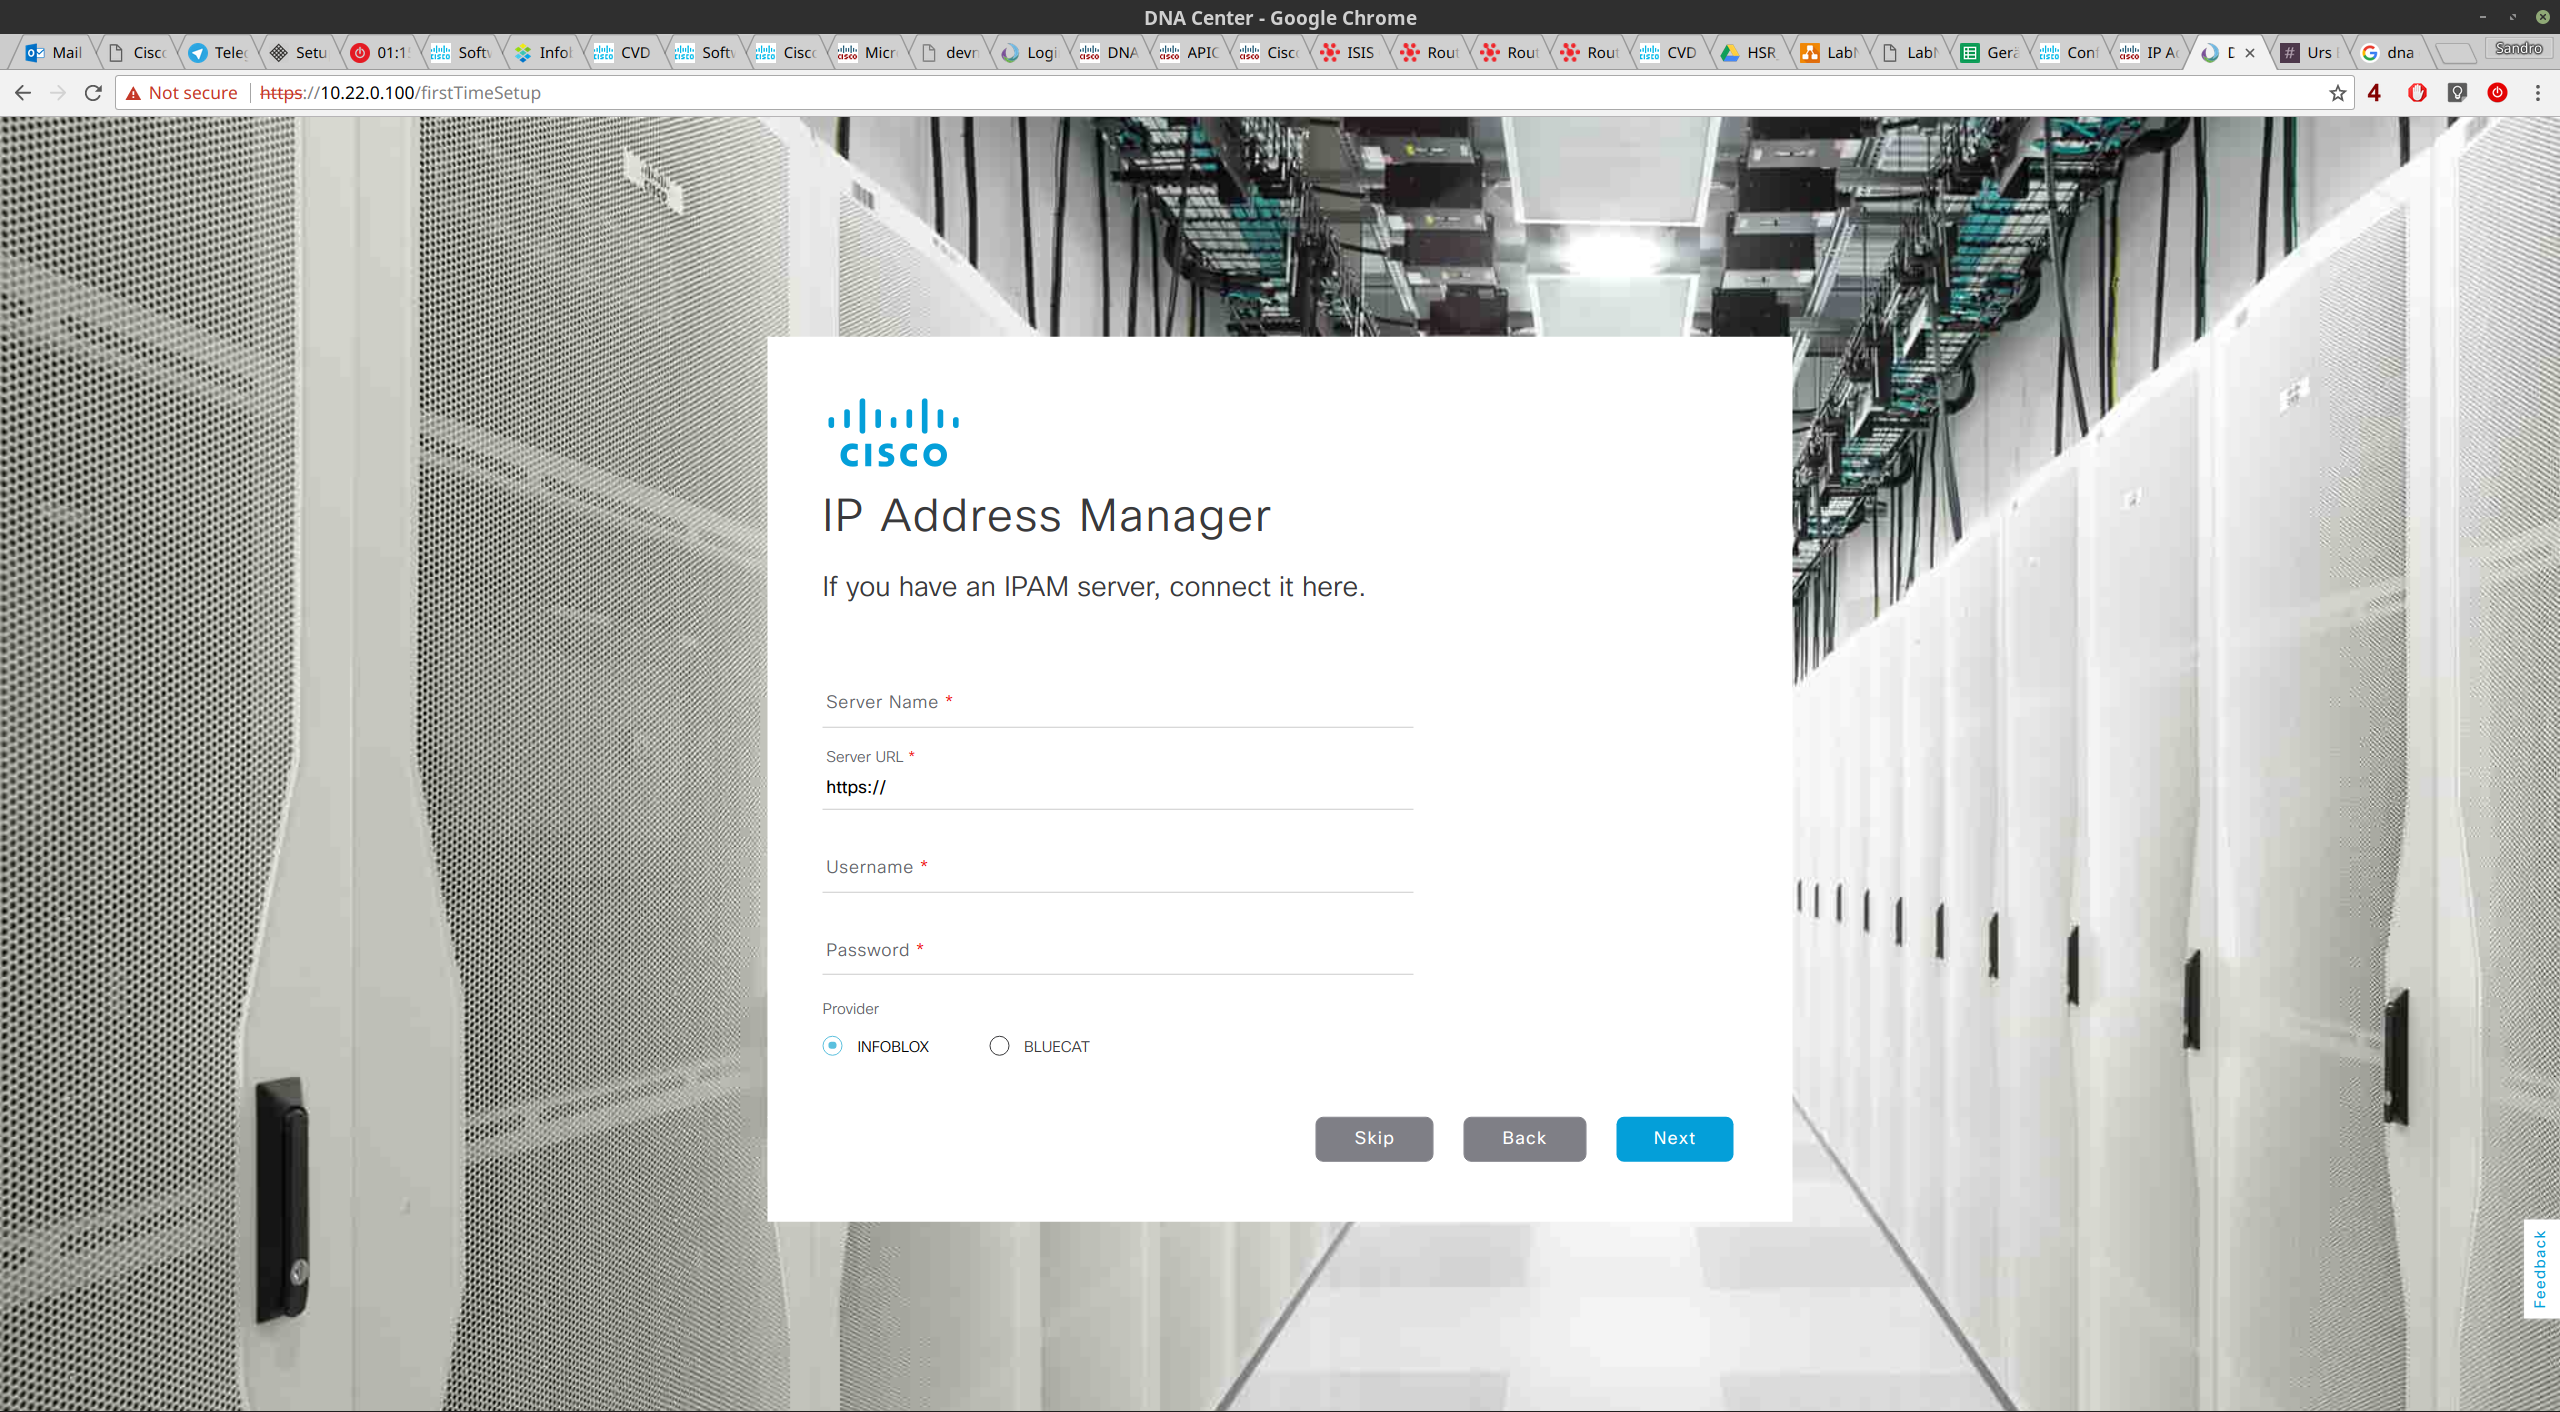
\includegraphics[height=9cm]{img/sc_007.png}
	\caption{DNA Center Web GUI - Cisco IPAM}
	\label{fig:dna-center-gui-3}
\end{figure}

Danach ist die initiale Konfiguration beendet und das DNA Center Dashboard wird angezeigt.

\begin{figure}[H]
	\centering
	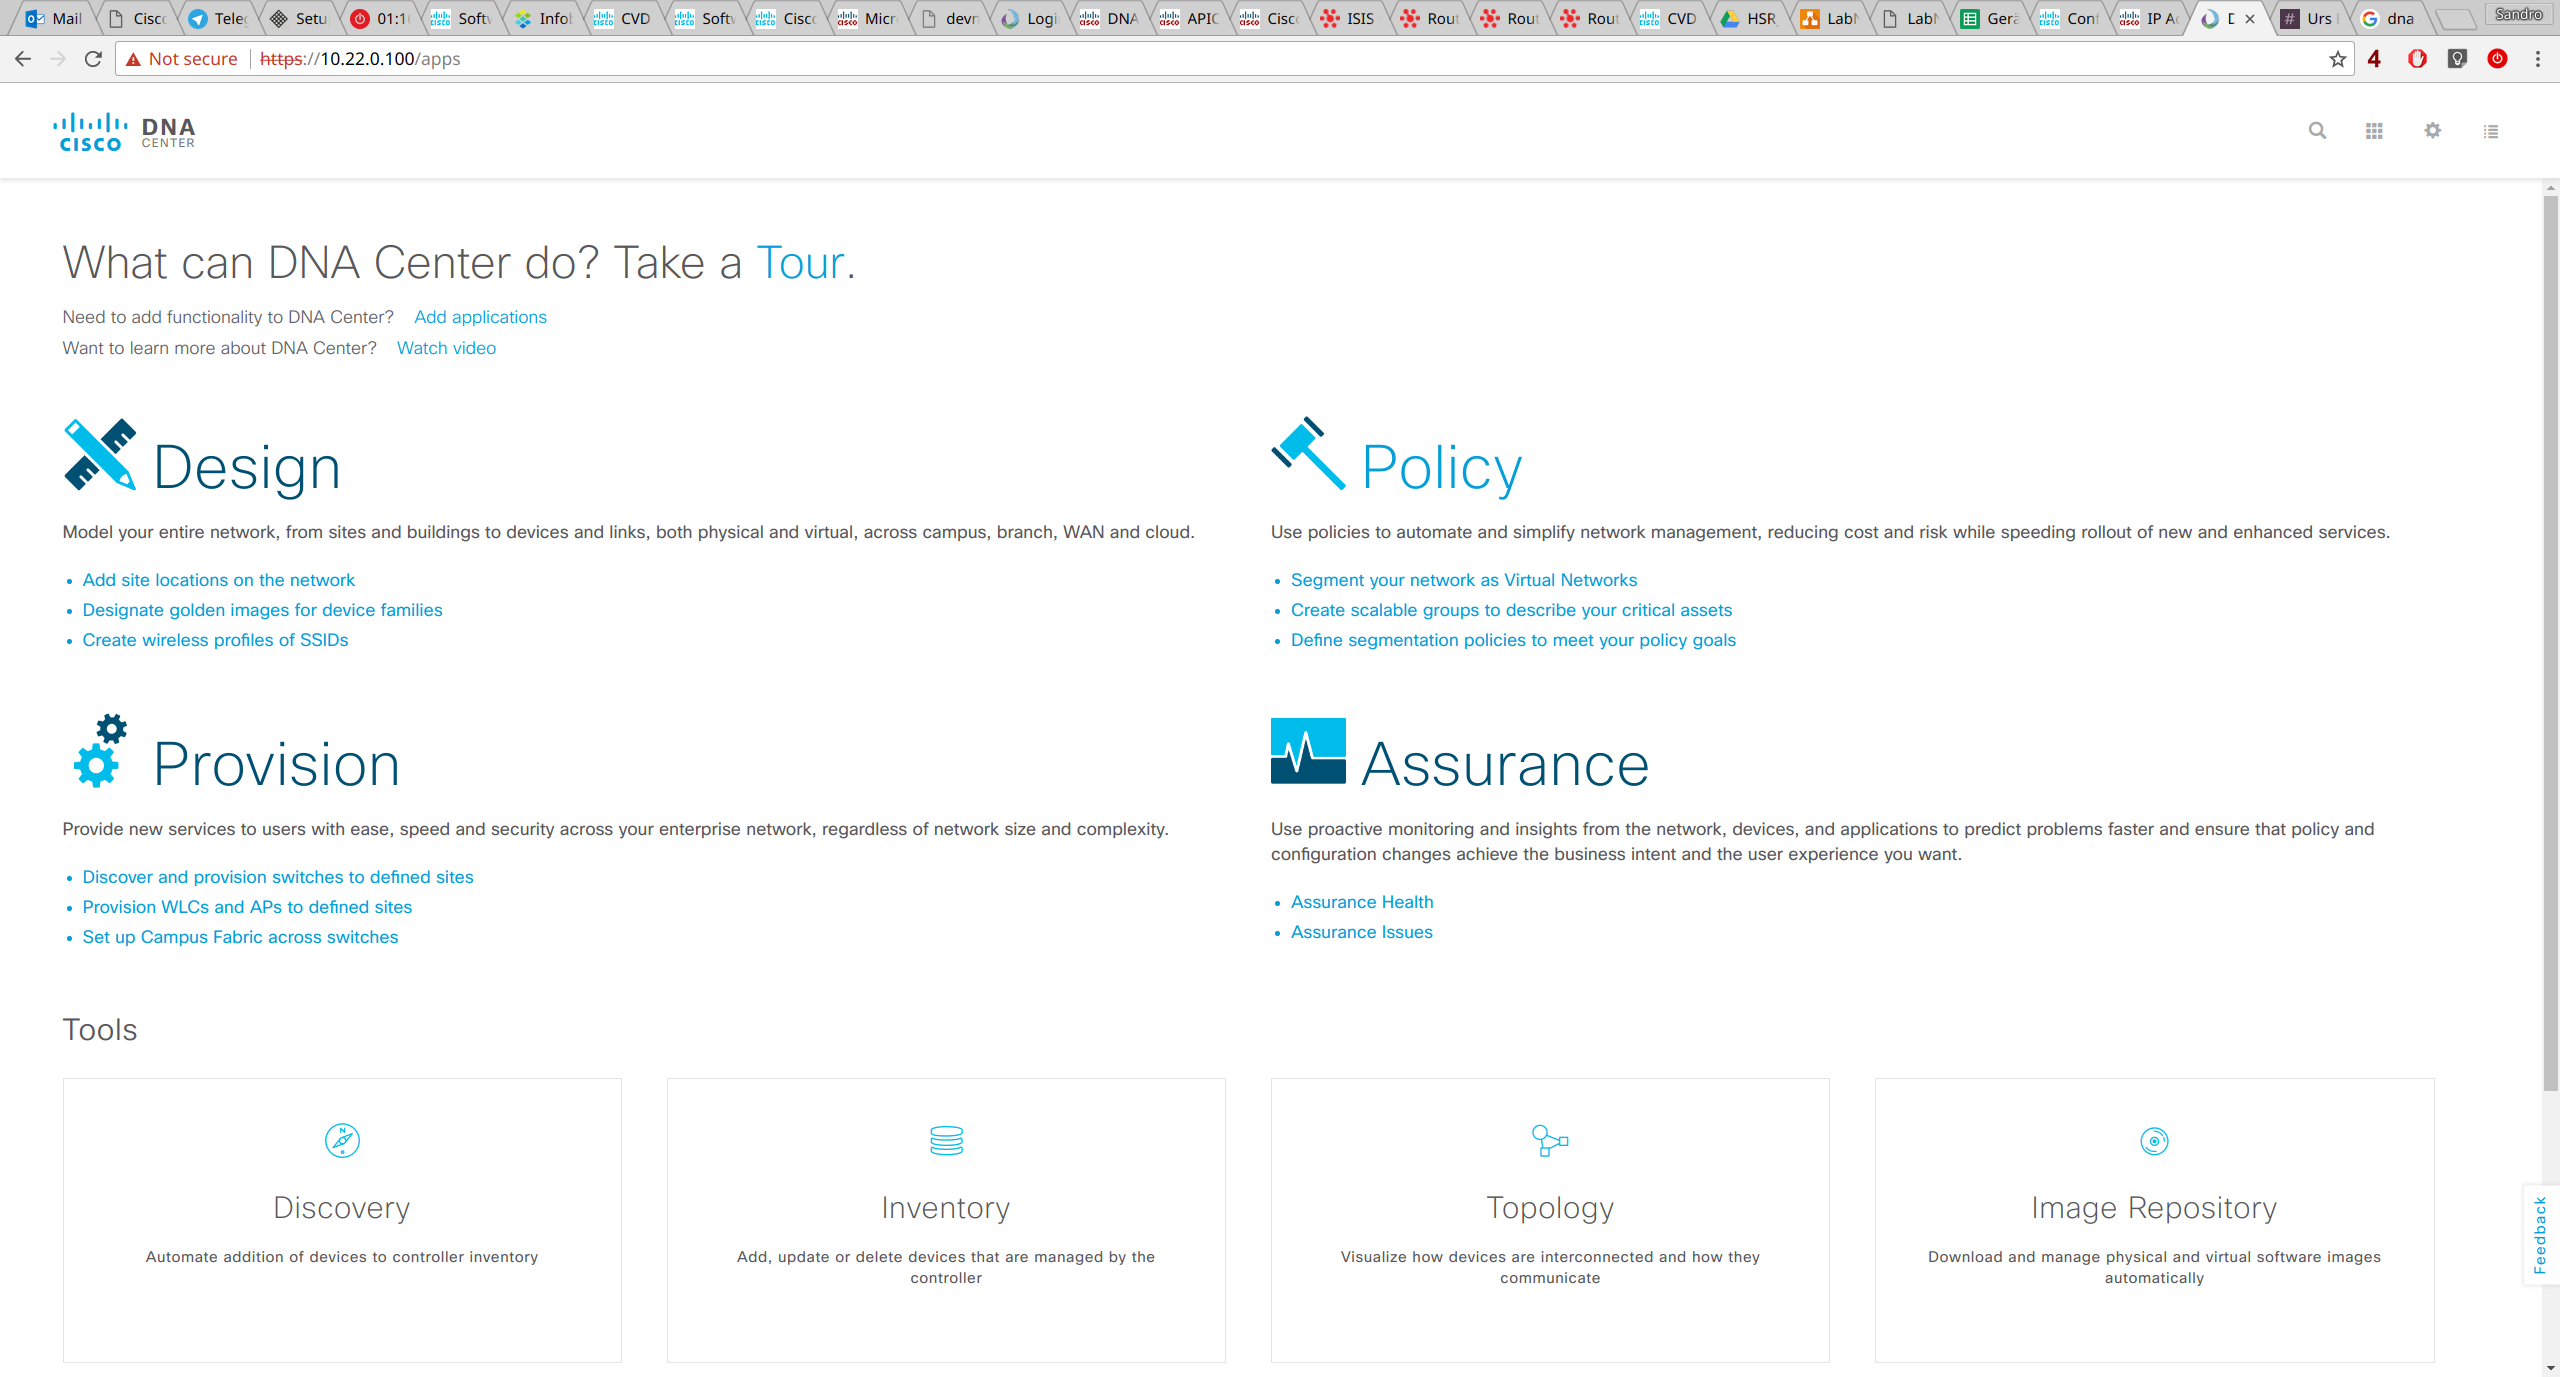
\includegraphics[height=9cm]{img/sc_008.png}
	\caption{DNA Center Web GUI - Dashboard}
	\label{fig:dna-center-gui-4}
\end{figure}

\subsection{DNA Center Updates}
Da sich das DNA Center während dem Setup Prozess nicht automatisch aktualisiert und die DNA Center Versionen in relativ kurzen Intervallen released werden, ist es ratsam, gleich zu Beginn die aktuellsten Updates zu installieren.

Der Updateprozess birgt jedoch einige Hürden:
\begin{itemize}
	\item System Updates müssen vor den Package Updates heruntergeladen und installiert werden.
	\subitem Werden die Package Updates vor dem System Update ausgeführt, können diese blockieren. 
	\item Die Package Updates müssen in der richten Reihenfolge installiert werden.
	\item Die oben genannte Reihenfolge ist nicht direkt ersichtlich.
	\item Der Updatevorgang dauert mehrere Stunden.
	\item Der Updatefortschritt wird nicht angezeigt. 
	\item Während dem Updateprozess können Teile des Web-GUIs Fehlermeldungen anzeigen oder überhaupt nicht mehr erreichbar sein.\\
\end{itemize} 

Die Update Ansicht ist unter \textit{Einstellungen (Zahnrad-Symbol) $\rightarrow$ System Settings  $\rightarrow$ App Management} zu finden:

\begin{figure}[H]
	\centering
	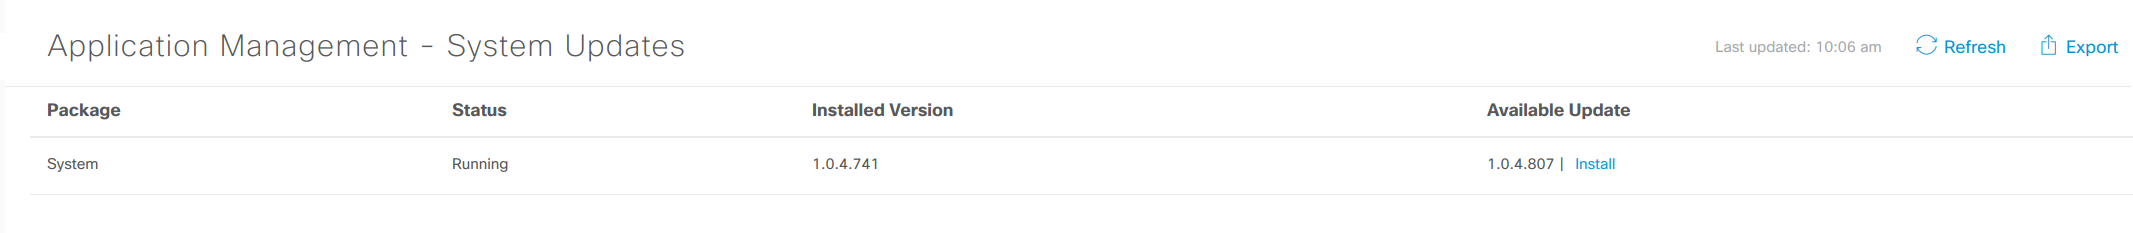
\includegraphics[width=\columnwidth]{img/sc_009.png}
	\caption{DNA Center App Management}
	\label{fig:dna-center-gui-update-1}
\end{figure}

\subsubsection{Fehlgeschlagene Updates reparieren}
Falls Updates in der falschen Reihenfolge installiert wurden oder aus anderen Gründen blockiert sind, können bereits heruntergeladene oder installierte Updates mit folgenden Befehlen entfernt und bereinigt werden.
(am Beispiel von main-system-package:1.0.4.779):

\begin{lstlisting}[language=bash]
$ maglev package status | awk  '$3 ~ /[0-9]+/ {print $1":"$3}' | 
grep -v "^system" |  while read pkg; 
do maglev catalog package delete $pkg;done
$ maglev system_update_package install main-system-package:1.0.4.779
\end{lstlisting}

\subsubsection{Update Reihenfolge}
Nach einem Update wurde die Reihenfolge von System und Package Updates angepasst. Vermutlich um den Administrator dazu zu bringen zuerst die System Updates zu installieren. 

\begin{figure}[H]
	\centering
	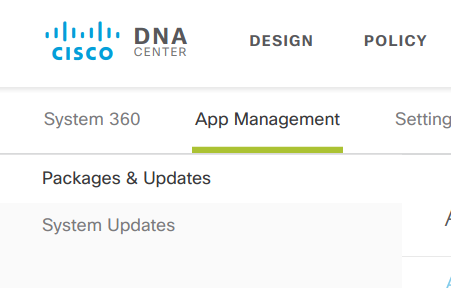
\includegraphics[height=4cm]{img/sc_010.png}
	\caption{DNA Center App Management - Alte Menü Anordnung}
	\label{fig:dna-center-gui-update-2}
\end{figure}

\subsubsection{Schwierigkeit: CCO Credentials für Updates notwendig}

Application Packages und System Updates können nur installiert werden, wenn die CCO Credentials hinterlegt sind.

\begin{figure}[H]
	\centering
	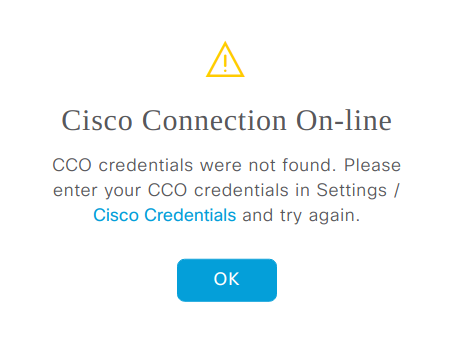
\includegraphics[height=4cm]{img/dan-center-cisco-credentials-required.png}
	\caption{DNA Center Upgrade - Cisco Credentials required}
	\label{fig:dna-center-cisco-credentials-required}
\end{figure}

\subsubsection{Schwierigkeit: Unterschiedliche Versionsangabe}

Beim Updatevorgang kann es zu Verwirrungen kommen, weil die Versionangabe von der Funktion \textit{About} von der Version des System Packages abweicht.

\begin{figure}[H]
	\centering
	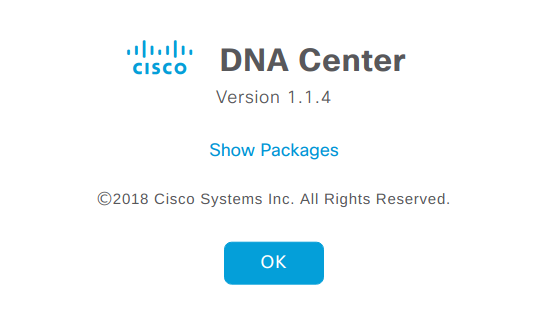
\includegraphics[height=3cm]{img/dna-center-about.png}
	\caption{DNA Center - About - Version}
	\label{fig:dna-center-about}
\end{figure}

Oben wurde bei \textit{About} die richtige Version 1.1.4 angegeben. Nachfolgend die Anzeige unter \textit{System Updates}, welche eine andere Version anzeigt.
\begin{figure}[H]
	\centering
	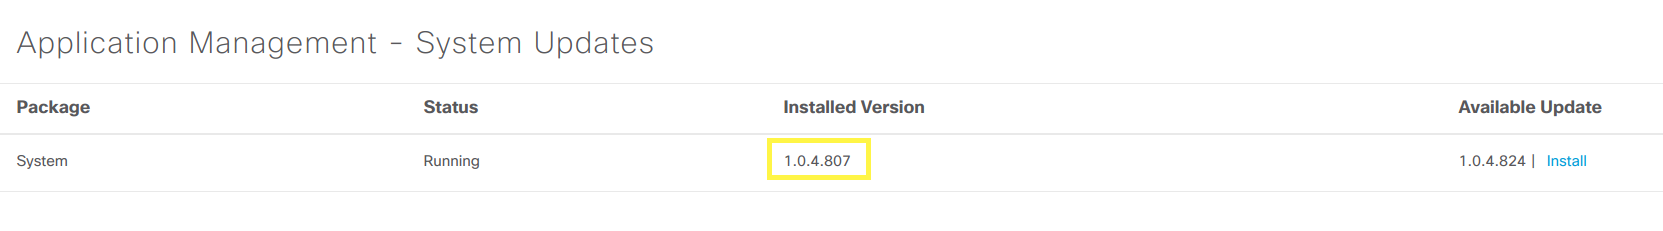
\includegraphics[height=2.25cm]{img/dna-center-system-upgrade-version.png}
	\caption{DNA Center - System Upgrade - Version}
	\label{fig:dna-center-system-upgrade}
\end{figure}

\subsection{DNA Center Netzwerk Design}

\subsubsection{Network Hierarchy}

Gemäss unserer Netzwerk Architektur wie in Kapitel \ref{fig:LabNetworkArchitecture} beschrieben, haben wir zwei Standorte. Rapperswil mit zwei Gebäuden und Jona mit einem Gebäude.
In DNA Center können diese sehr einfach im Abschnitt \textit{Design $\rightarrow$ Network Hierarchy} hinzugefügt werden. 

\begin{figure}[H]
	\centering
	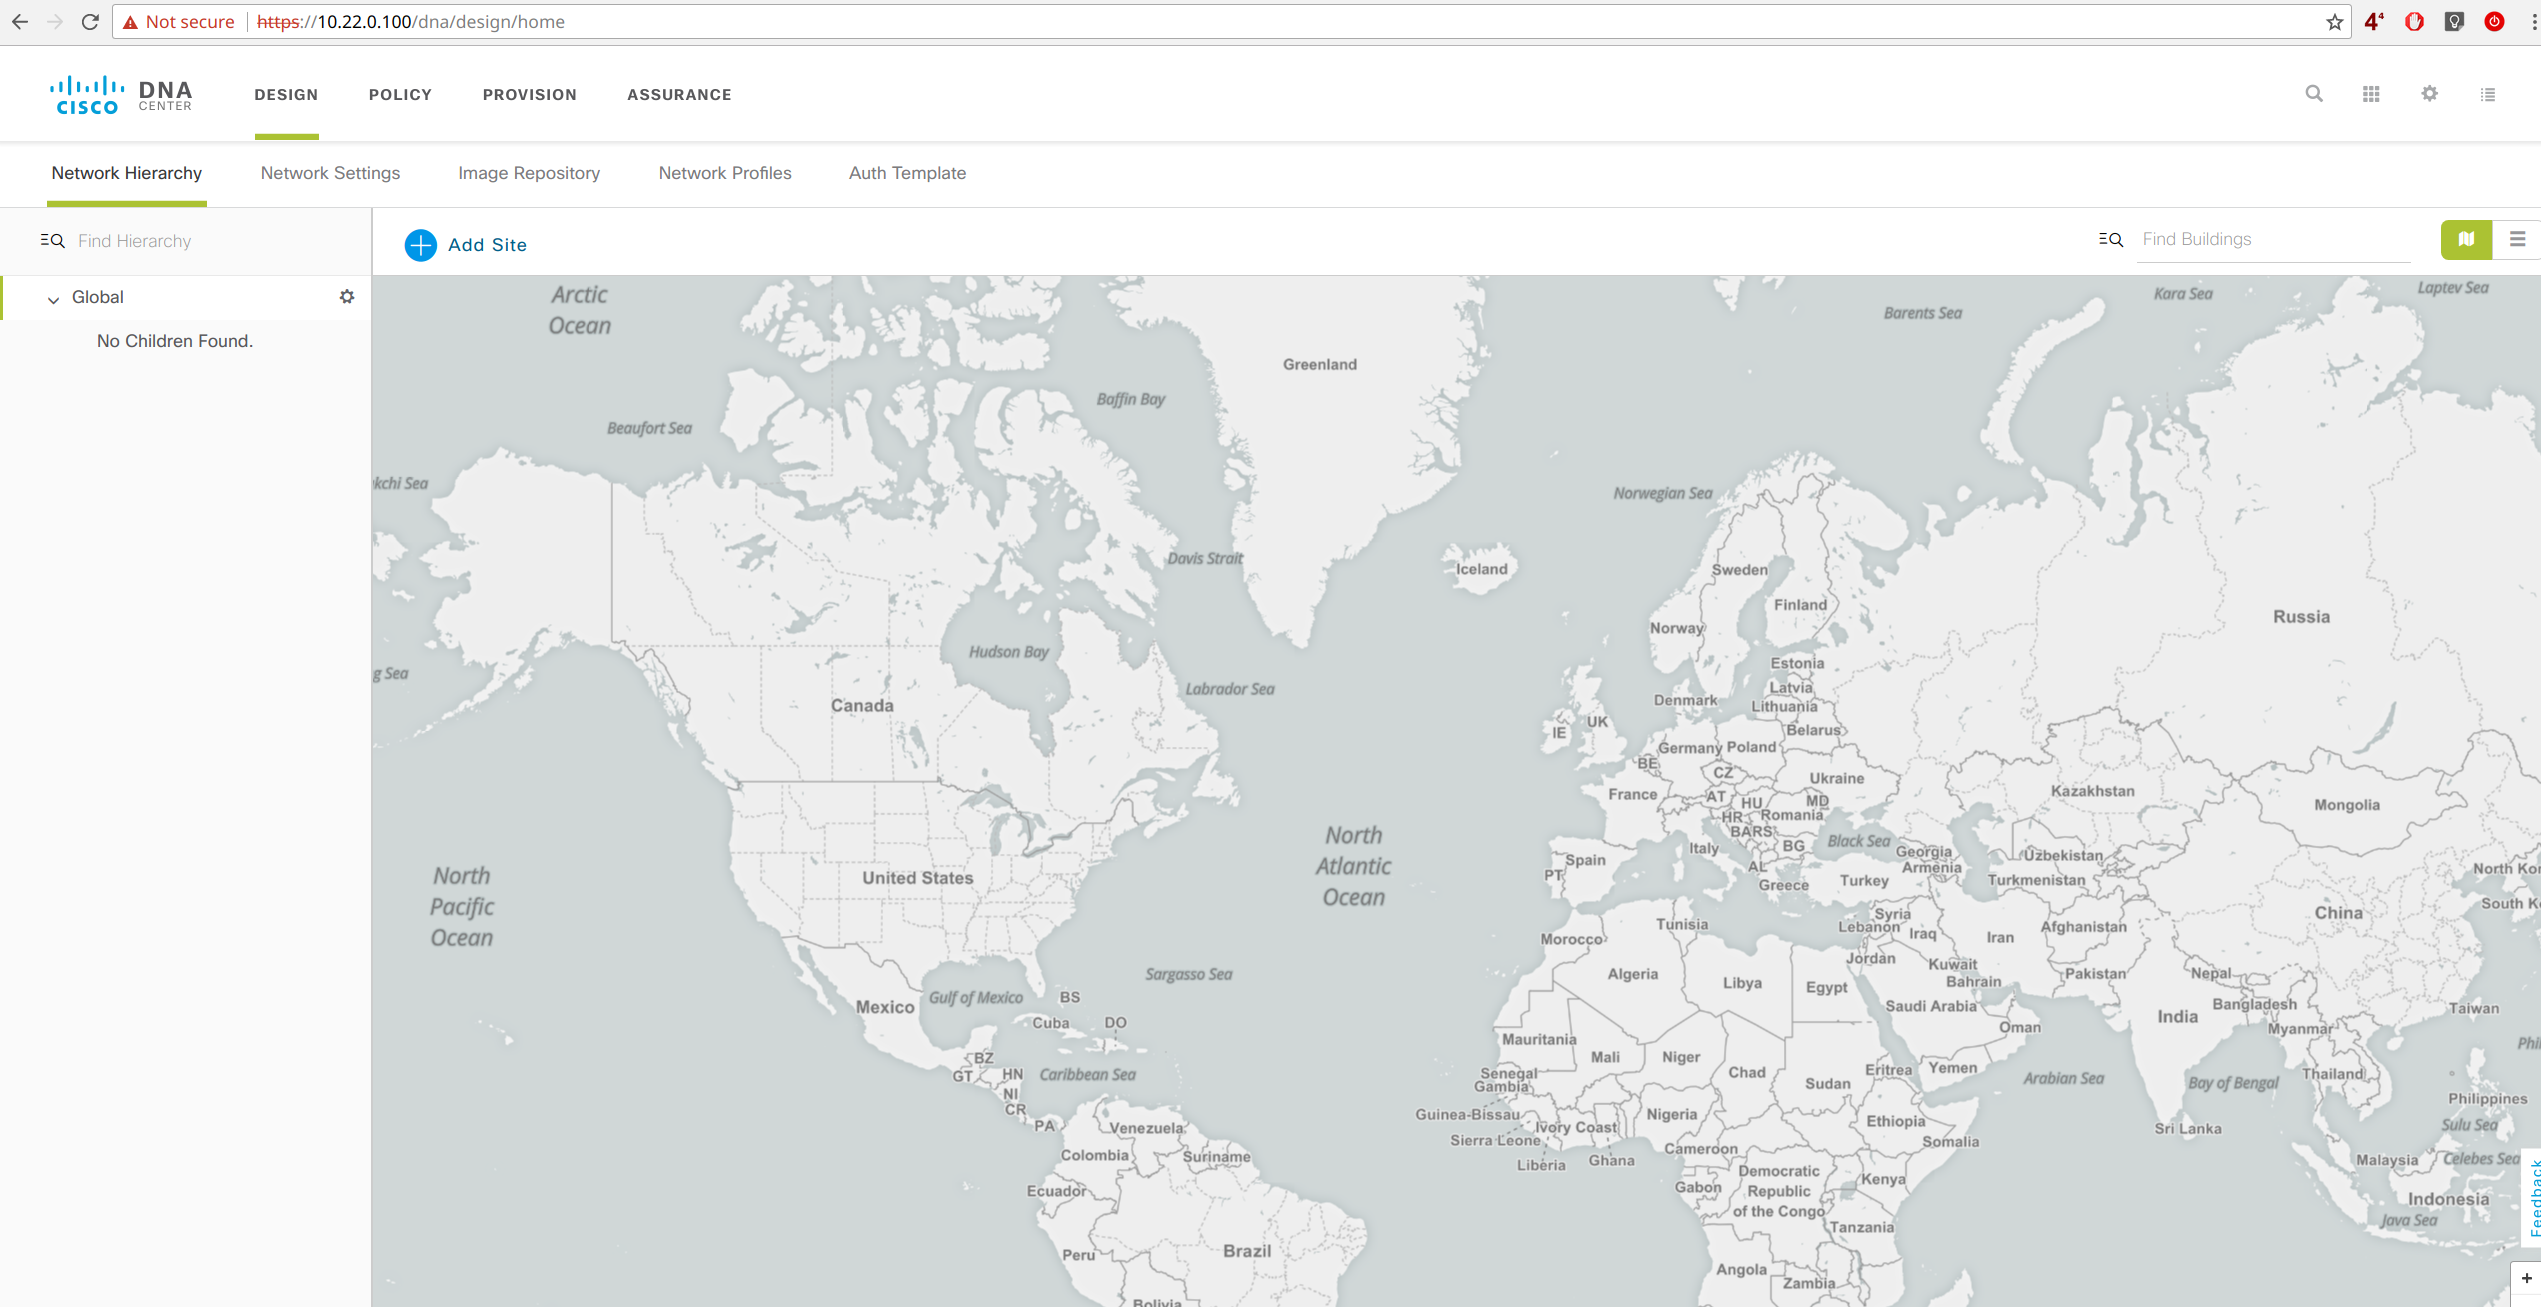
\includegraphics[height=8cm]{img/Selection_011.png}
	\caption{DNA Center Design Map}
	\label{fig:dna-center-design-1}
\end{figure}

\begin{figure}[H]
	\centering
	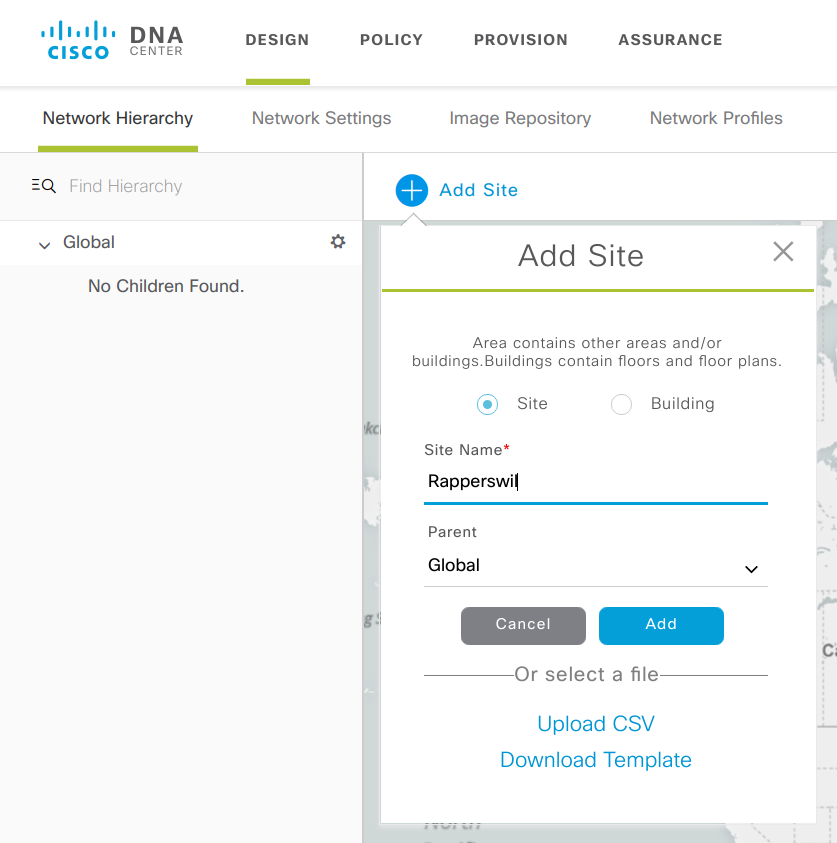
\includegraphics[height=6cm]{img/Selection_012.png}
	\caption{DNA Center Design - Standort hinzufügen}
	\label{fig:dna-center-design-2}
\end{figure}

\begin{figure}[H]
	\centering
	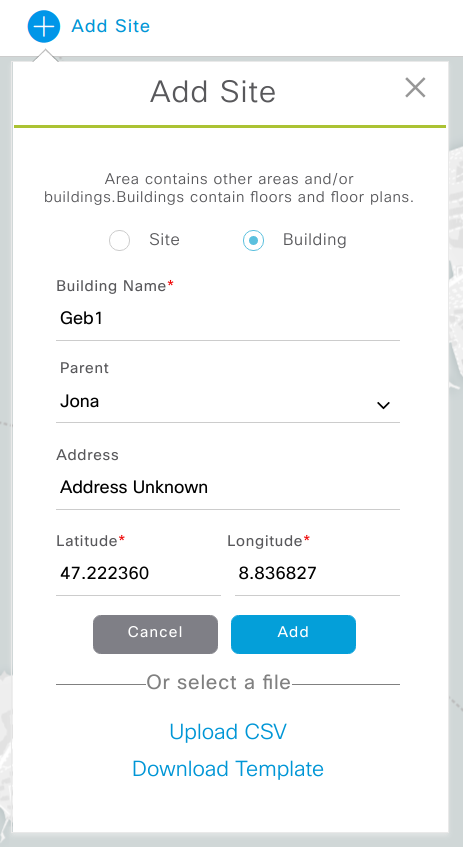
\includegraphics[height=6cm]{img/Selection_014.png}
	\caption{DNA Center Design - Gebäude können mit Koordinaten hinzugefügt werden.}
	\label{fig:dna-center-design-3}
\end{figure}

\begin{figure}[H]
	\centering
	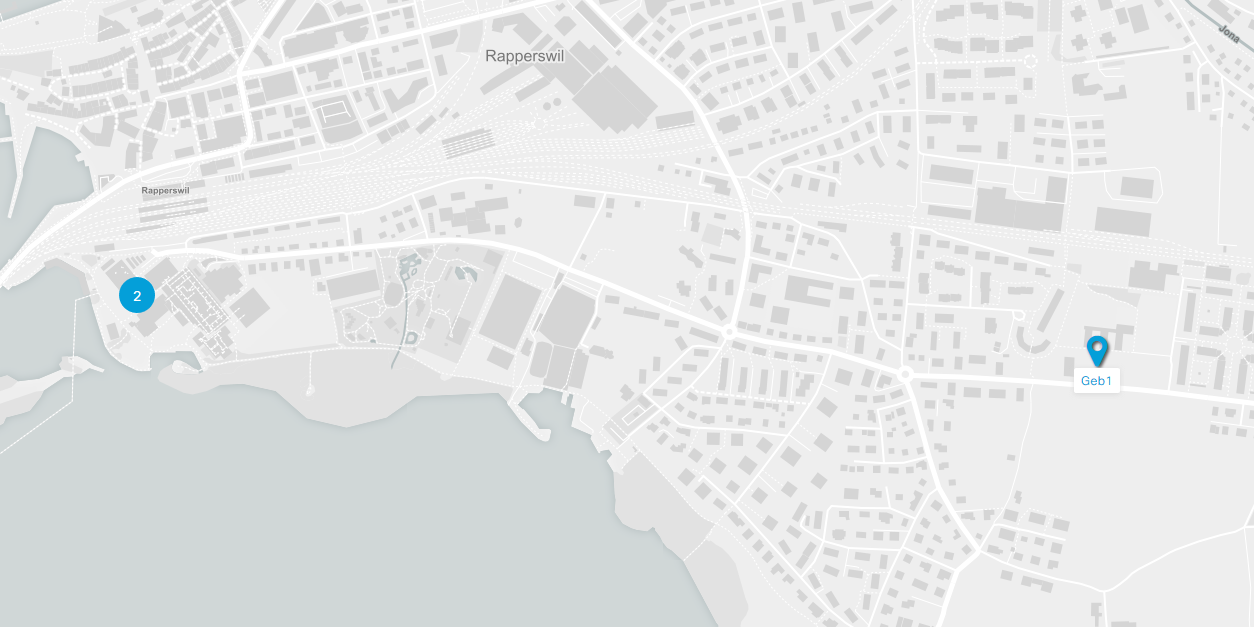
\includegraphics[height=8cm]{img/design_map_overview.PNG}
	\caption{DNA Center Design - Übersicht über alle Standorte und Gebäude}
	\label{fig:dna-center-design-overview}
\end{figure}

\subsection{LAN Automation}
Das DNA Center nutzt Plug and Play um automatisch Netzwerkgeräte in Betrieb zu nehmen und initial zu konfigurieren.
 
\subsubsection{DHCP Konfiguration}
Bei unserem ersten Versuch ein Seed-Device festzulegen, wurde vom DNA Center kein DHCP Server konfiguriert, weshalb wir diesen manuell auf Infoblox eingerichtet haben.\\


Cisco PnP kann über die DHCP Optionen 43 und 60 konfiguriert werden (siehe \cite{cisco-pnp-dhcp}). In unserem Fall haben wir diese Optionen wie nachfolgend auf der Grafik erischtlich auf dem Infoblox Server konfiguriert. Diese sind nötig, damit das Netzwerkgerät den PnP Server findet.

\begin{figure}[H]
	\centering
	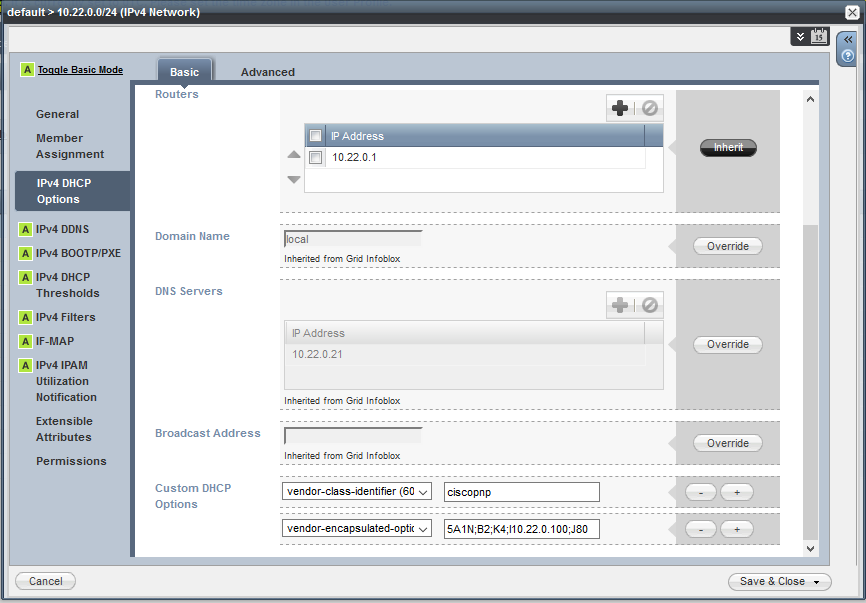
\includegraphics[height=10cm]{img/Infoblox_PNP.png}
	\caption{Infoblox Cisco PNP DHCP Option Konfiguration}
	\label{fig:cisco-pnp}
\end{figure}

Mit diesen Einstellungen hat PnP funktioniert. Allerdings nur sehr unzuverlässig und es kam oft zu Problemen, weshalb dies für viele Geräte mehrmals wiederholt werden musste. Hier ist zu empfehlen, nie mehr als ein Gerät gleichzeitig in Betrieb zu nehmen, damit es möglichst wenig Probleme gibt.

\begin{figure}[H]
	\centering
	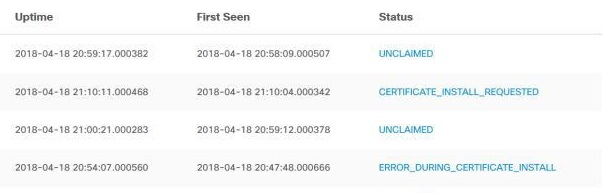
\includegraphics[height=4cm]{img/DNA_Center_Unclaimed_Errors_1.PNG}
	\caption{DNA Center Provision - Fehlermeldungen in der "Unclaimed List"}
	\label{fig:dna-center-provision-unclaimed-2}
\end{figure}
\subsection{Underlay Konfiguration}

Das ISIS Routing im Underlay sollte vom DNA Center automatisch konfiguriert werden können. Da die entsprechende Funktion LAN Automation in unserem Versuch aber nicht funktionierte, wurde der Underlay manuell konfiguriert. Dazu wurden auf den Geräten IP Addressen auf den Loopback Interfaces und den P2P Links konfiguriert und entsprechende Router eingerichtet. Am Border wurde BGP verwendet, damit die Devices auch aus dem Legacy Netz erreichbar sind.\\
Dabei ist uns aufgefallen, dass die Geräte nur über eine IP-Base Lizenz verfügen. Für die Verwendung von BGP und VRF-lite ist aber die IP-Services Lizenz nötig. 

\begin{figure}[H]
	\centering
	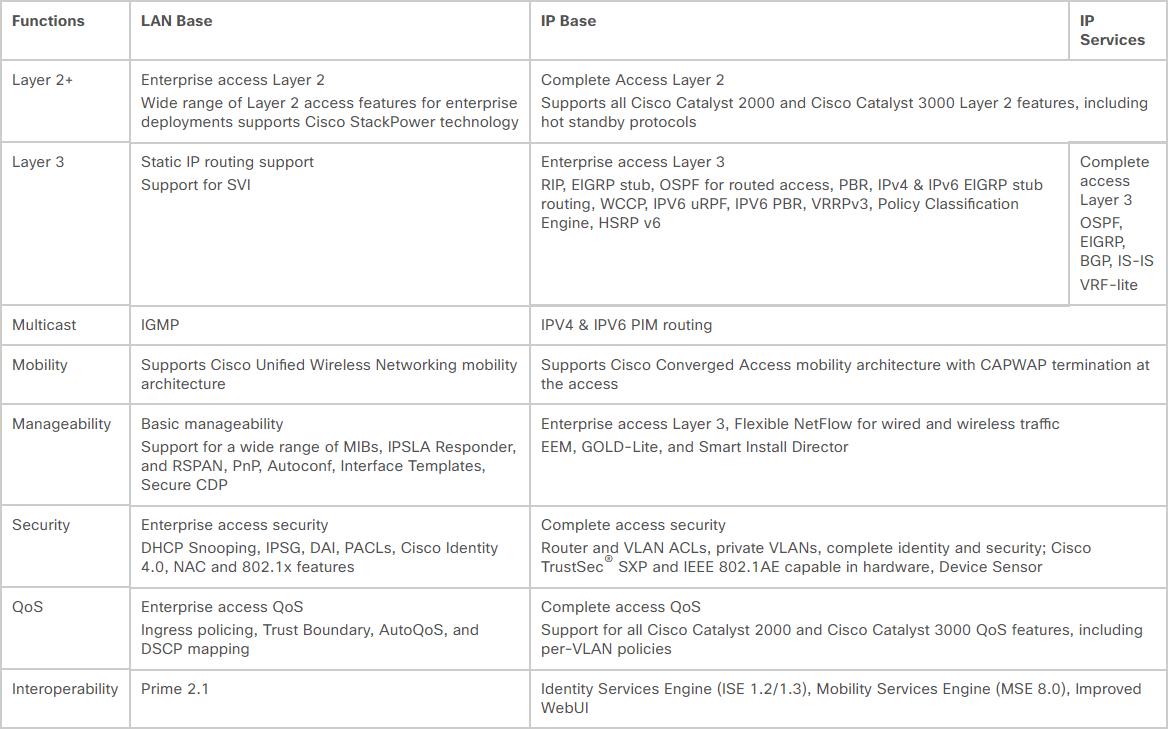
\includegraphics[width=16cm]{img/IPBaseServices.png}
	\caption{IP Base and Services}
	\label{fig:IP Base and Services Licences}
\end{figure}

Mit folgenden Befehlen war es möglich, eine IP-Services Test Lizenz zu aktivieren und somit die benötigten Features zu nutzen.

\begin{lstlisting}[language=bash]
sh license right-to-use activate ipservices all accepptEULA
reload
show license right-to-use
\end{lstlisting}

\subsection{"Claim" von Netzwerkgeräten}

\subsubsection{DNA Center Provision - Unclaimed Devices}

Nachdem die Geräte via PnP eine initiale Konfiguration erhalten haben und die Konnektivität via ISIS und BGP sichergestellt war, wurden diese im Device Inventory als Unclaimed Devices angezeigt.

\begin{figure}[H]
	\centering
	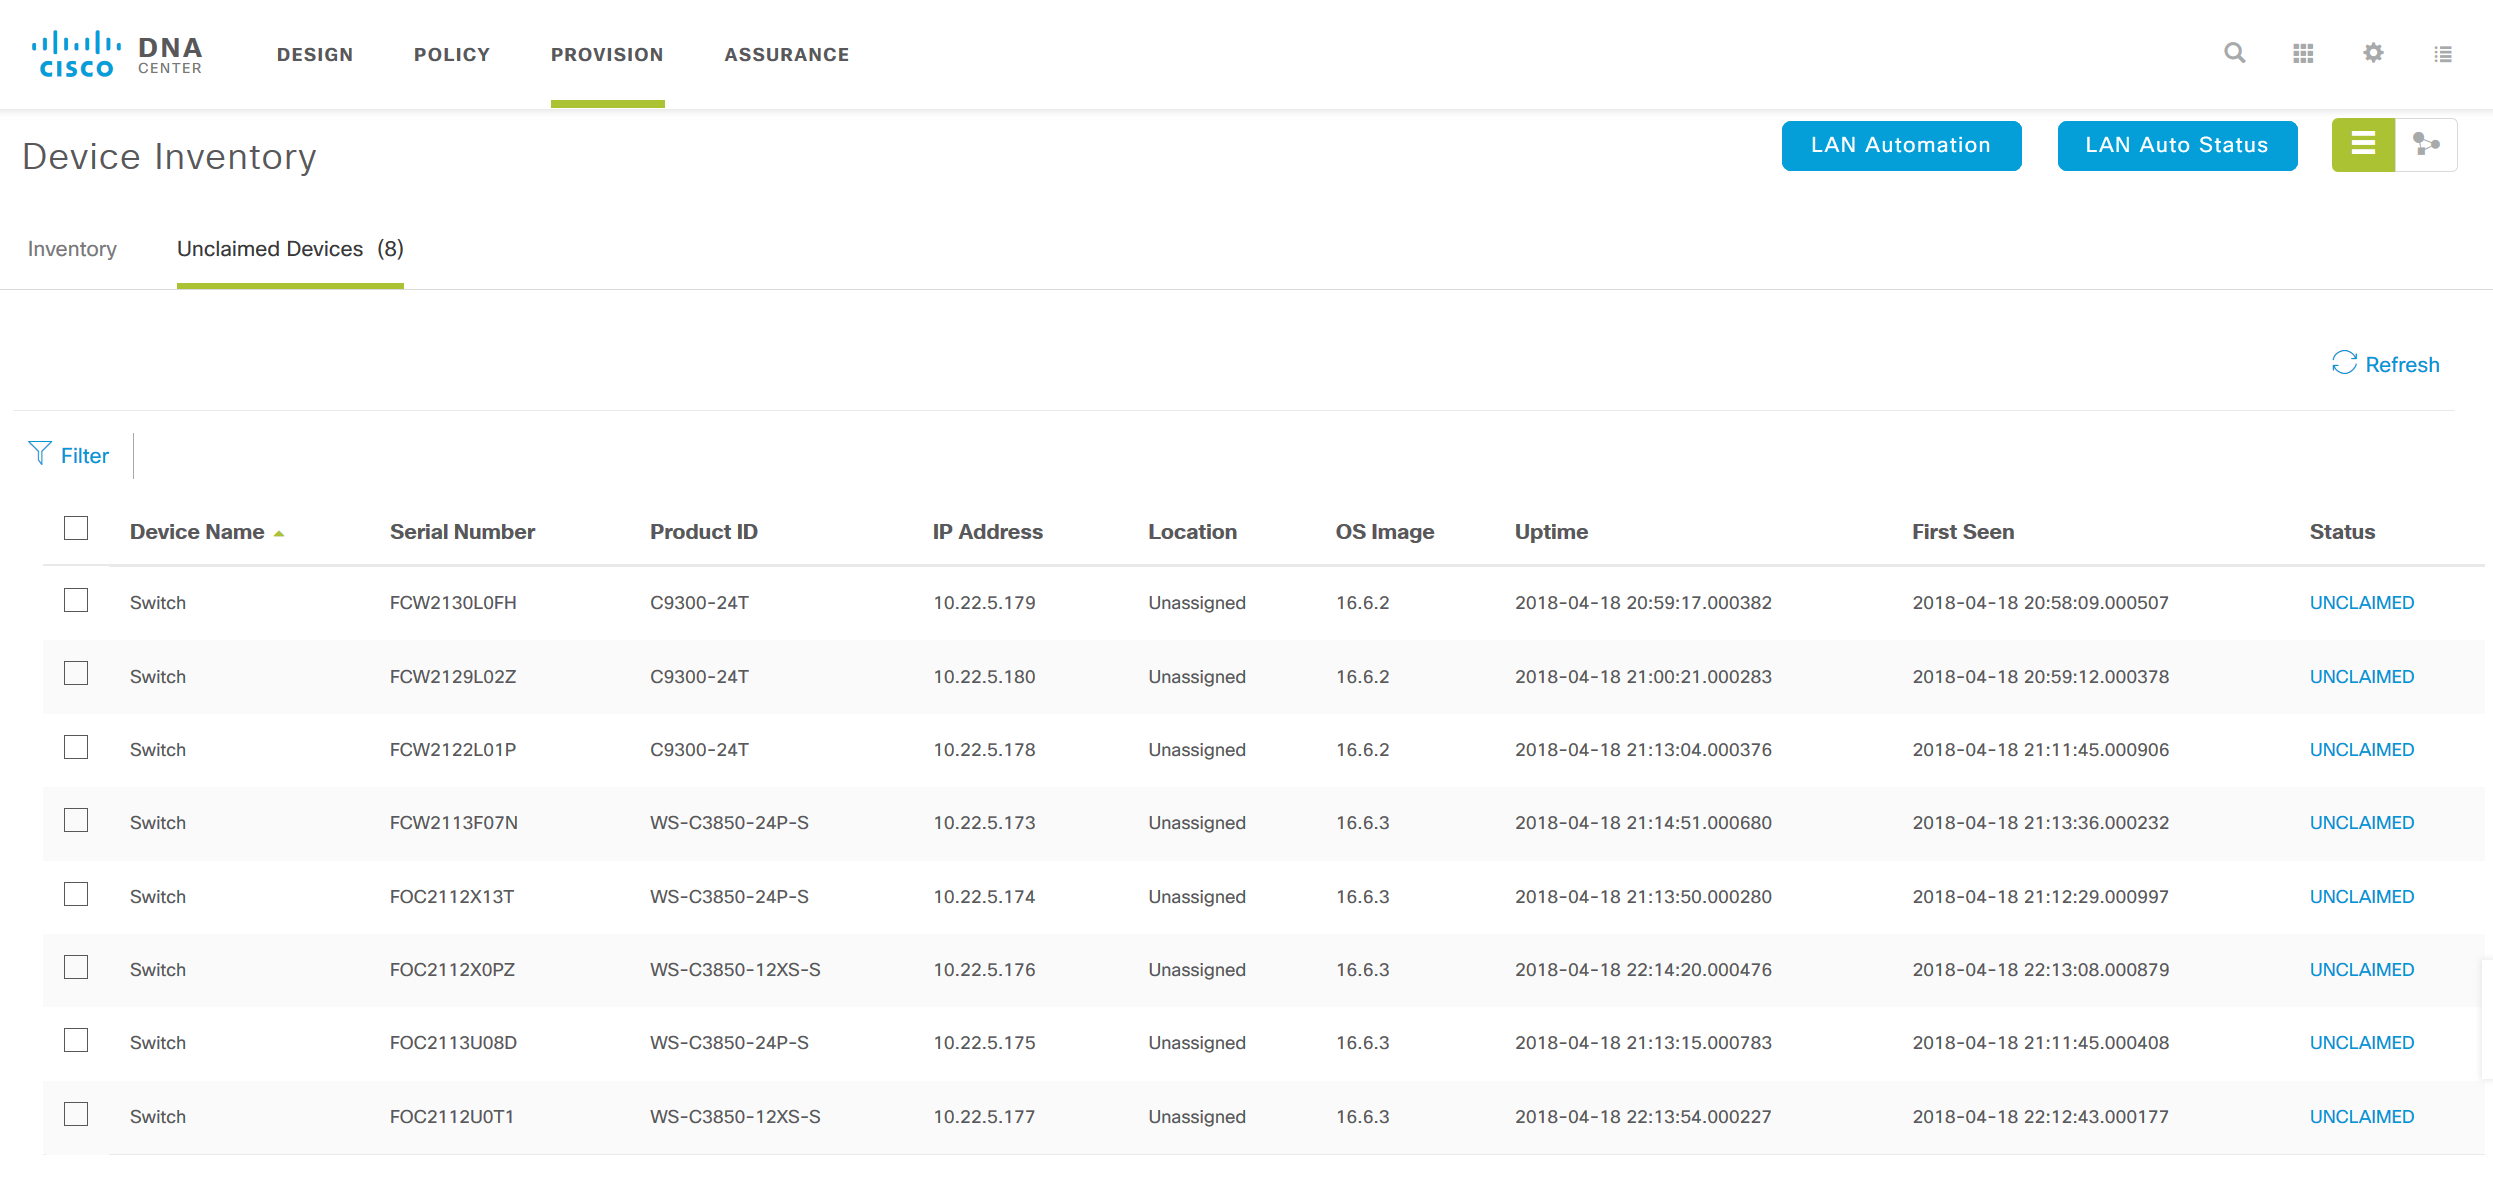
\includegraphics[height=8cm]{img/DNA_Center_All_Fabric2_Unclaimed.PNG}
	\caption{DNA Center Provision - Alle Geräte erfolgreich in der "Unclaimed List"}
	\label{fig:dna-center-provision-unclaimed}
\end{figure} 


\subsection{Netzwerkgeräte zu Inventory hinzufügen}

Der nächste Schritt wäre nun, die Devices zu "Claimen". Dies bedeutet, dass die Geräte einem Standort zugewiesen werden und somit erste Konfigurationen erhalten können. Der Claim Prozess hat leider gar nie funktioniert. Das DNA Center reagierte einfach nicht auf die Eingabe.

\subsubsection{Manuell Geräte im DNA Center hinzufügen}
Da alle Versuche die Geräte automatisch hinzuzufügen gescheitert sind, entschieden wir uns den Vorgang manuell durchzuführen. 

Im Dashboard klickt man dazu auf \textit{Inventory} (siehe \ref{fig:dna-center-inventory-button})

\begin{figure}[H]
	\centering
	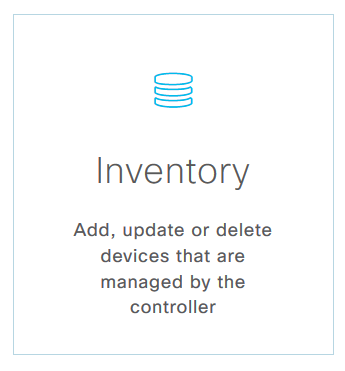
\includegraphics[height=3cm]{img/dna-center-inventory-button.PNG}
	\caption{DNA Center Dashboard - Inventory Knopf}
	\label{fig:dna-center-inventory-button}
\end{figure}

Anschliessend wählt man \textit{Add} (siehe \ref{fig:dna-center-inventory-add})

\begin{figure}[H]
	\centering
	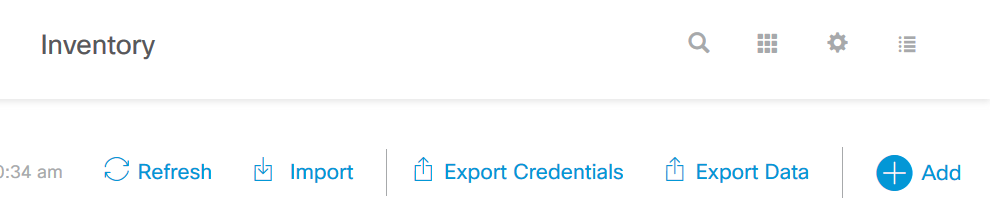
\includegraphics[height=3cm]{img/dna-center-inventory-add.PNG}
	\caption{DNA Center Inventory - Gerät hinzufügen}
	\label{fig:dna-center-inventory-add}
\end{figure}

Danach müssen folgende Informationen eingegeben werden:

\begin{itemize}
	\item Device Type
	\item Device IP \ Name
	\item SNMP (Version, Read und Write Community)
	\item CLI (via SSH oder Telnet) \textit{oder}
	\item NETCONF
\end{itemize}

Wir entschieden uns hier CLI via SSH zu wählen.

\begin{figure}[H]
	\centering
	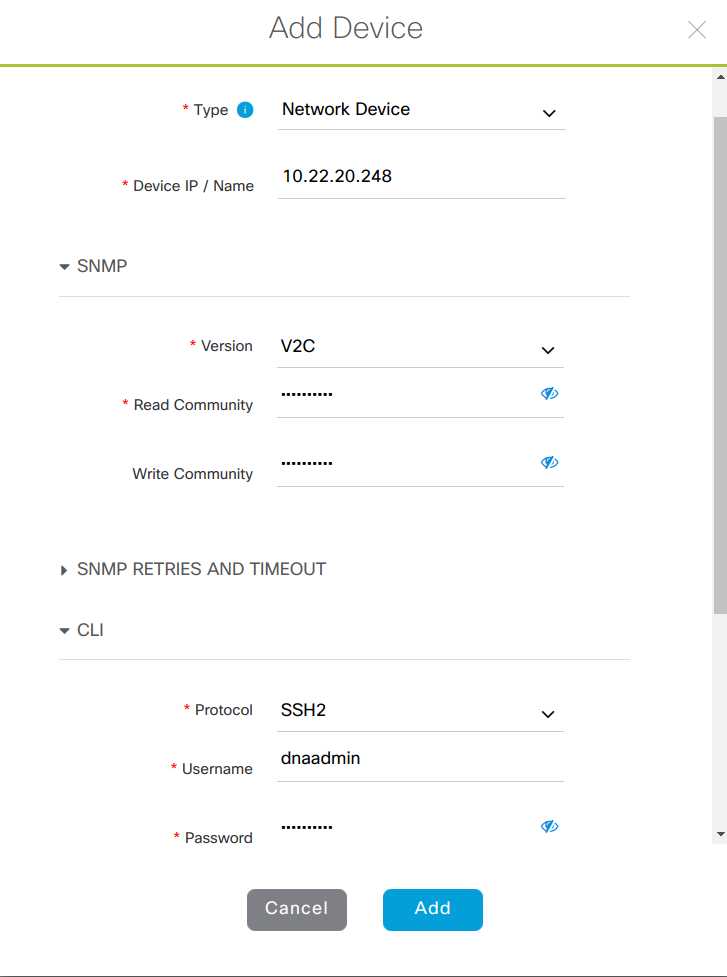
\includegraphics[height=5cm]{img/dna-center-inventory-add-form.png}
	\caption{DNA Center Inventory - Formular Gerät hinzufügen}
	\label{fig:dna-center-inventory-add-form}
\end{figure}

Danach erscheint das Gerät im Inventory. (siehe \ref{fig:dna-center-inventory-index-new})

\begin{figure}[H]
	\centering
	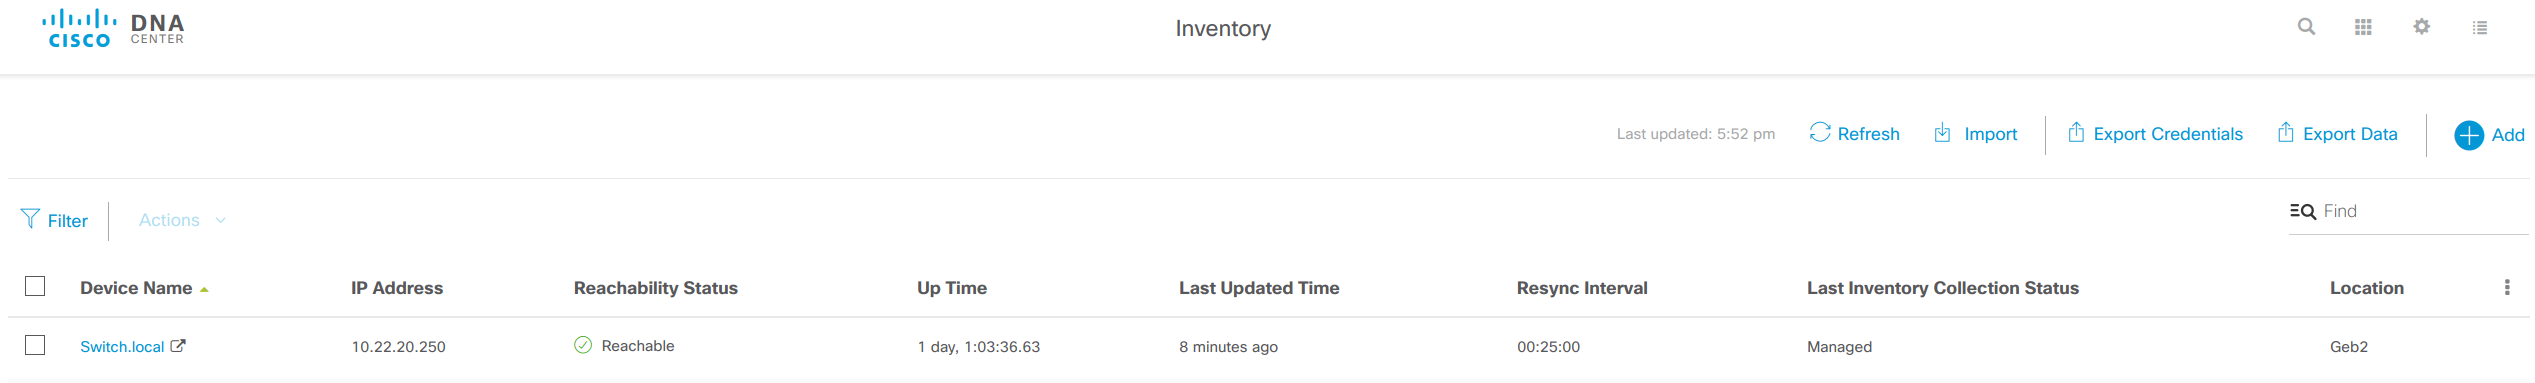
\includegraphics[height=2cm]{img/dna-center-inventory-index-new.png}
	\caption{DNA Center Inventory - Neue Geräte in der Liste}
	\label{fig:dna-center-inventory-index-new}
\end{figure}


\subsection{Image Repository}
Im DNA Center können Netzwerkgeräte automatisch aktualisiert werden. Sobald ein Gerät im Inventory erfolgreich hinzugefügt worden ist, sucht das DNA Center automatisch nach Updates. Allerdings nur, wenn ein CCO Account konfiguriert ist. Die verfügbaren Images sind unter \textit{Desing $\rightarrow$ Global $\rightarrow$ Image Repository} zu finden.

\begin{figure}[H]
	\centering
	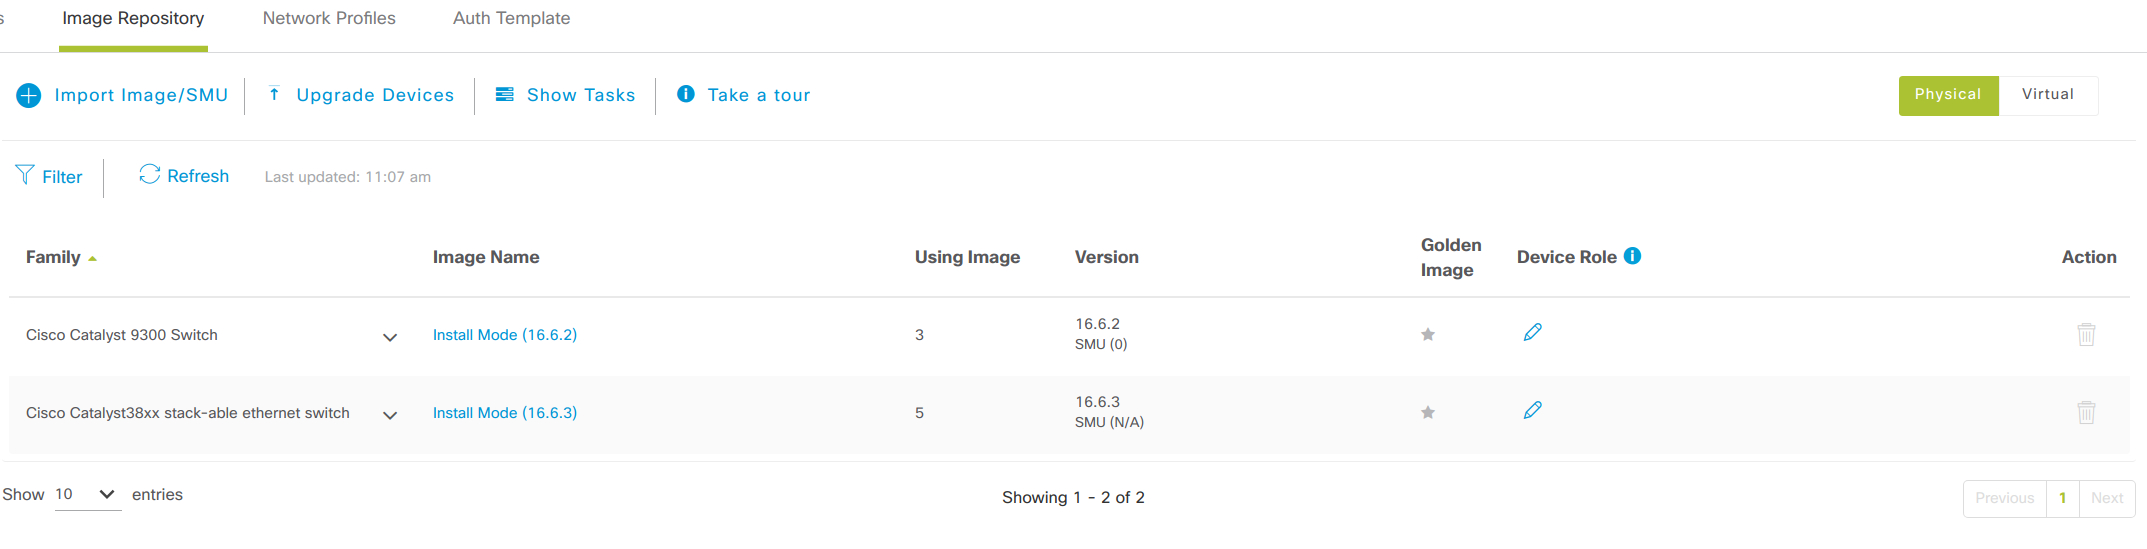
\includegraphics[height=2cm]{img/dna-center-design-image-repository.png}
	\caption{DNA Center Design - Image Respository}
	\label{fig:dna-center-design-image-repository}
\end{figure}

In diesem Image Repository kann das gewünschte Image mit einem "Golden Tag" versehen werden, worauf dieses heruntergeladen wird. 

\subsection{Automatisches Softwareupdate von Netzwerkgeräten}
Die Softwareupdates von Netzwerkgeräten können im DNA Center unter \textit{Provision $\rightarrow$ Devices $\rightarrow$ Inventory} durchgeführt werden. Ebenfalls wird hier angezeigt, welche Softwareversion zur Zeit auf dem Gerät installiert ist und ob diese aktuell ist.

\begin{figure}[H]
	\centering
	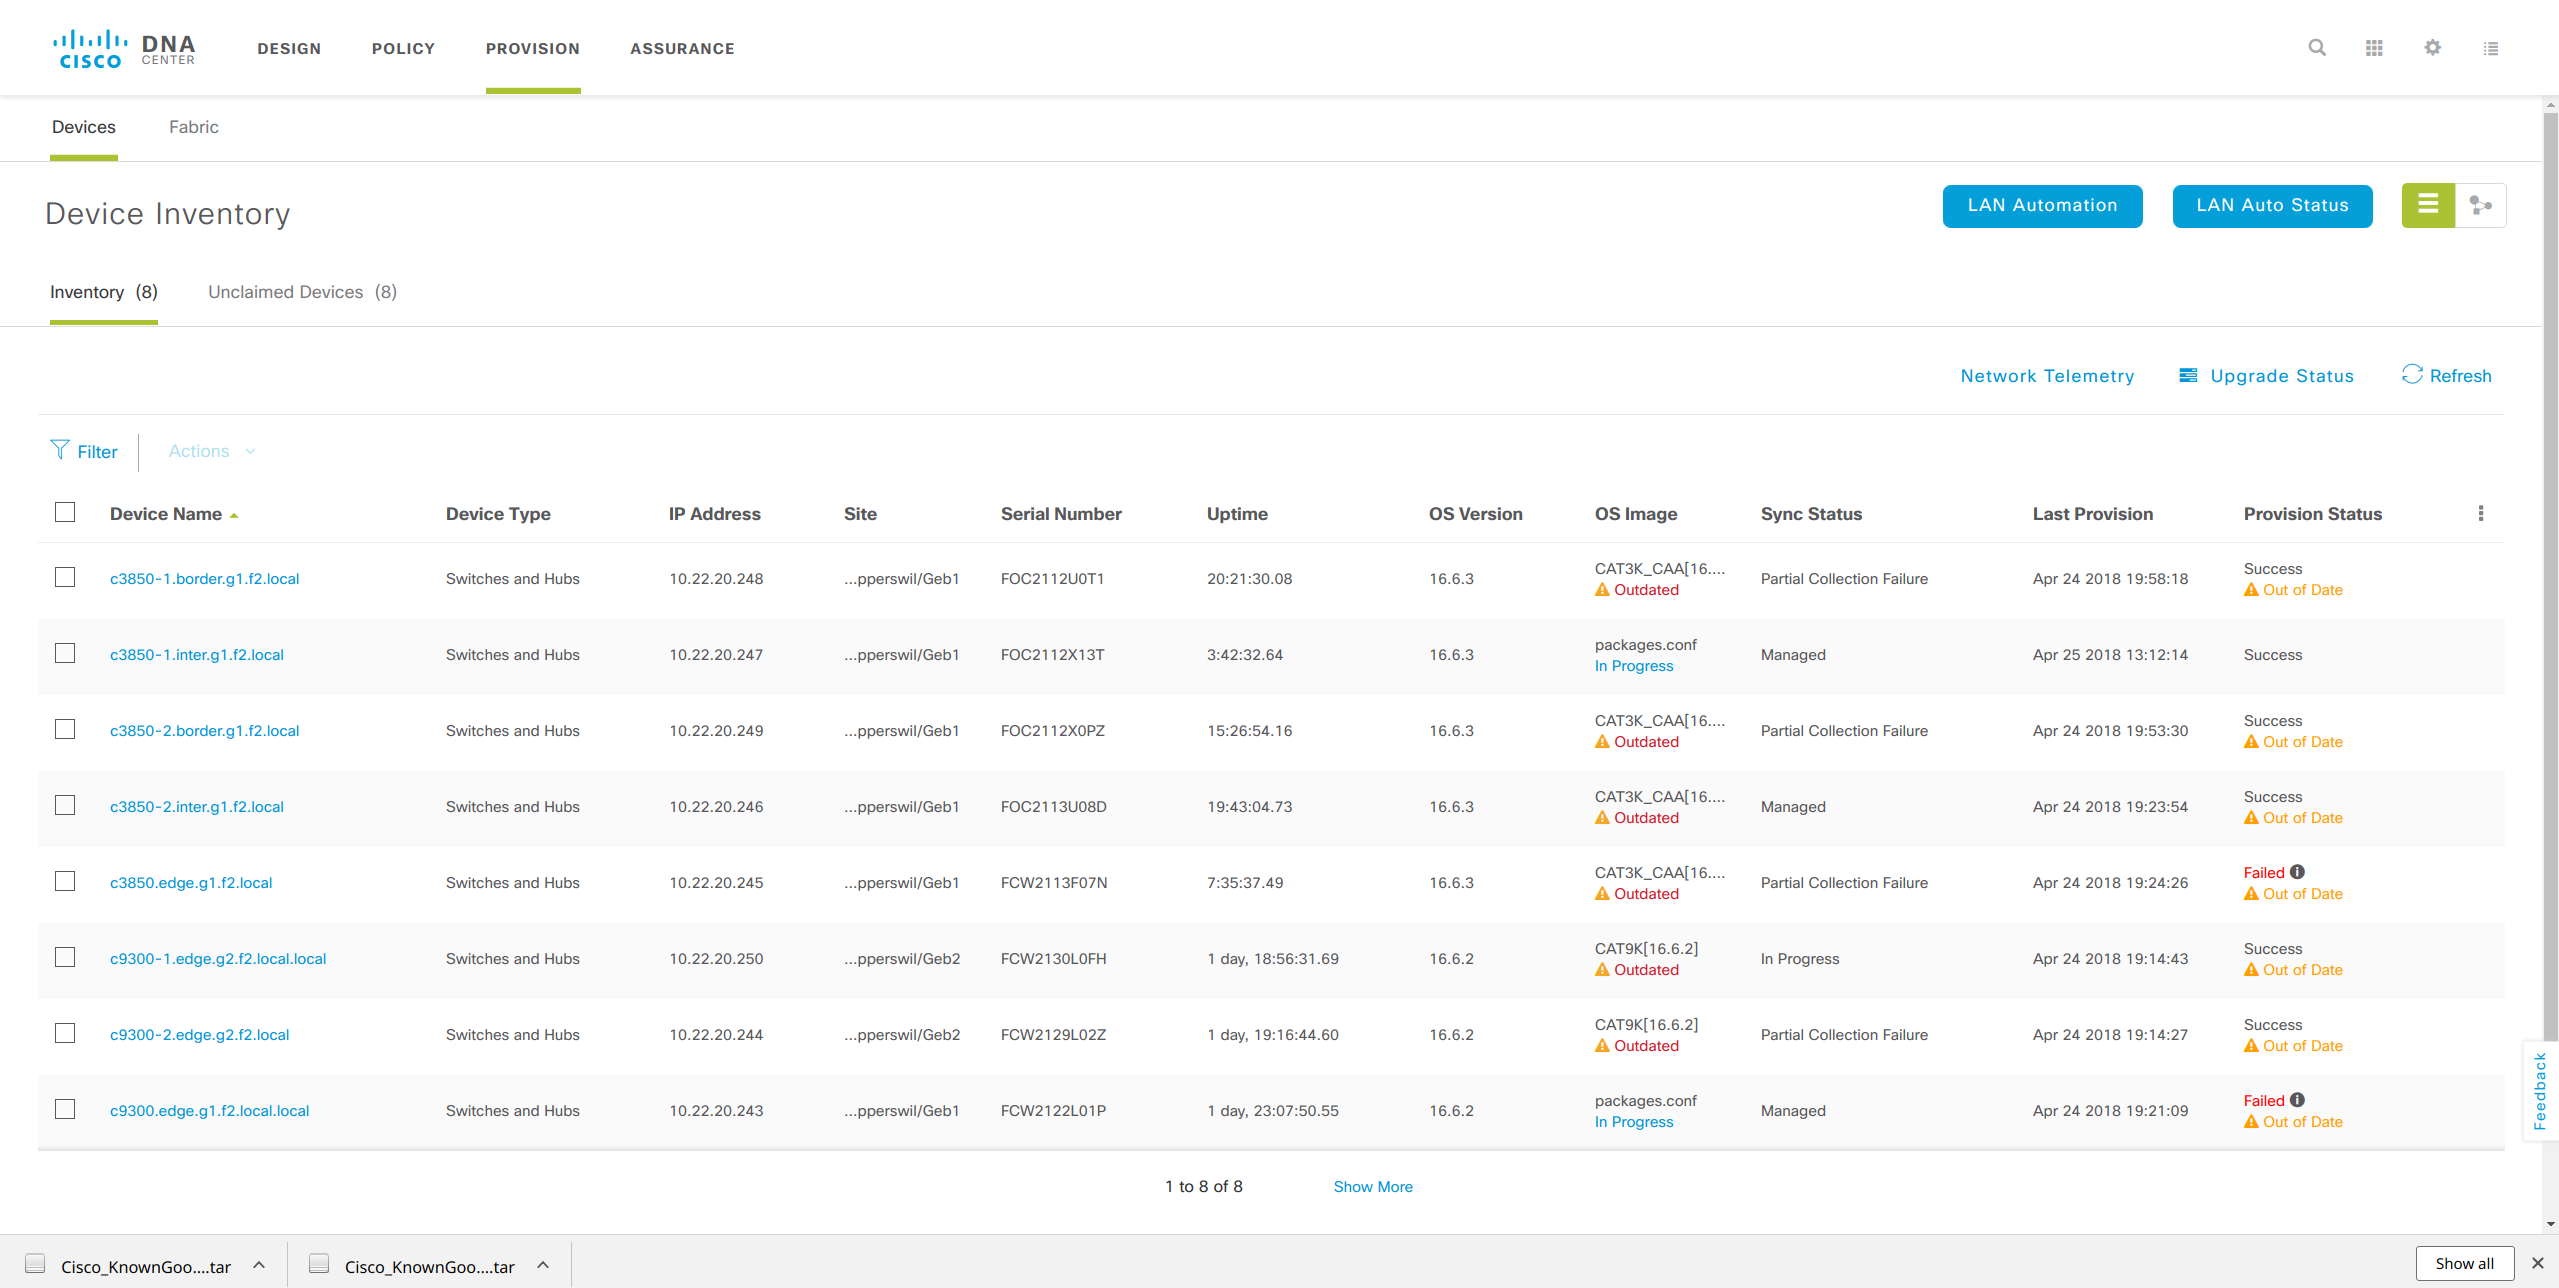
\includegraphics[height=8cm]{img/updates/Selection_070.png}
	\caption{DNA Center Provision - Die OS Versionen sind outdated.}
	\label{fig:dna-center-provision-updates}
\end{figure}

Das automatische Softwareupdate hat bei keinem von unseren Switches oder Routern geklappt. Nachfolgend eine kleine Übersicht über die verschiedenen Update Methoden und ausgeführten Versuche.

\begin{tabular}{ | l | l |}
	\hline
	\textbf{Methode} & \textbf{Resultat} \\
	\hline	
	\makecell{DNA Center über HTTP und SFTP} & Fehlgeschlagen (siehe \ref{fig:dna-center-provision-updates-1}) \\
	CLI - HTTPS    & Fehlgeschlagen (siehe \ref{fig:dna-center-provision-updates-2}) \\
	CLI - SCP      & Fehlgeschlagen (siehe \ref{fig:dna-center-provision-updates-3}) \\
	CLI - TFTP     & Erfolgreich (siehe \ref{fig:dna-center-provision-updates-4}) \\	
	\hline
\end{tabular}
\captionof{table}{Softwareupdate - Übersicht Methoden und ausgeführten Versuche}

Beim Versuch die Softwareupdates im DNA Center über HTTP oder SFTP durchzuführen, wurden folgende Fehlermeldungen angezeigt.

\begin{figure}[H]
	\centering
	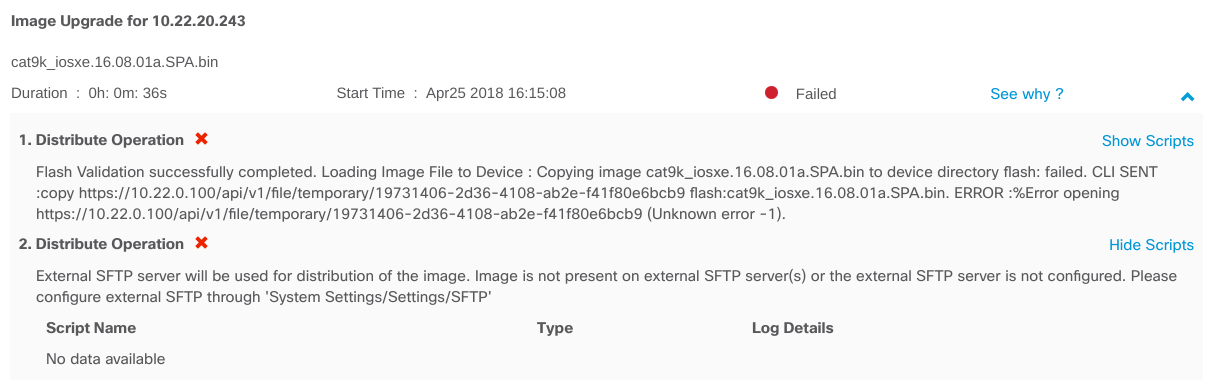
\includegraphics[height=5cm]{img/updates/Selection_071.png}
	\caption{Fehlermeldung Updatevorgang via DNA Center}
	\label{fig:dna-center-provision-updates-1}
\end{figure}

Die Upgrade Prozesse wurden schon beim Kopieren der einzelnen Images nach unterschiedlicher Dauer immer abgebrochen.

\subsection{Manuelles Softwareupdate}
Da wie oben beschrieben das automatische Update nicht funktionierte, wurde in einem nächsten Schritt versucht, die Updates manuell auf die Netzwerkgeräte zu installieren. 

\begin{figure}[H]
	\centering
	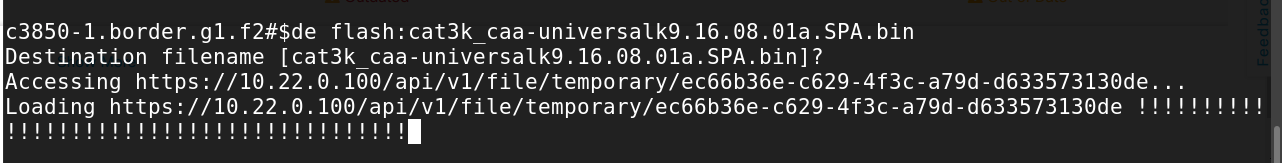
\includegraphics[height=2cm]{img/updates/Selection_082.png}
	\caption{Firmwareupdate Switch via CLI HTTPs}
	\label{fig:dna-center-provision-updates-2}
\end{figure}
Das Kopieren via HTTPS und SCP war sehr unzuverlässig und wurde nach einer gewissen Dauer abgebrochen.

\begin{figure}[H]
	\centering
	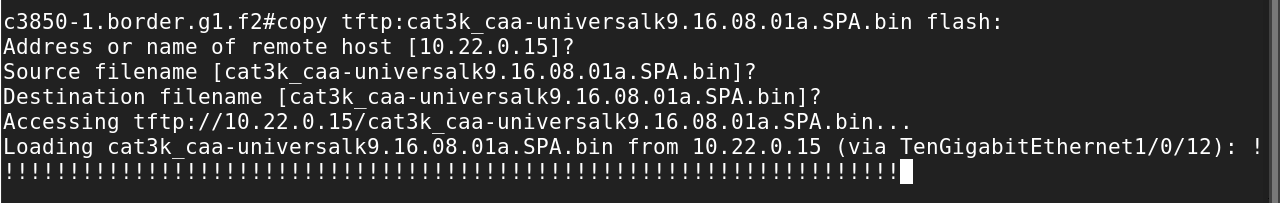
\includegraphics[height=2cm]{img/updates/Selection_111.png}
	\caption{Firmwareupdate Switch via CLI TFTP}
	\label{fig:dna-center-provision-updates-4}
\end{figure}
Mittels TFTP Server konnten die Devices schlussendlich erfolgreich aktualisiert werden.

\subsection{Lizenzen}
Die Lizenzen bezieht das DNA Center vom konfigurierten CCO Account. 
\begin{figure}[H]
	\centering
	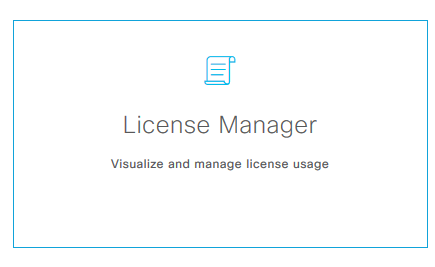
\includegraphics[height=3cm]{img/LicenceManager_001.png}
	\caption{Der Licence Manager ist über das Dashboard erreichbar.}
	\label{fig:dna-center-licence-1}
\end{figure}

\begin{figure}[H]
	\centering
	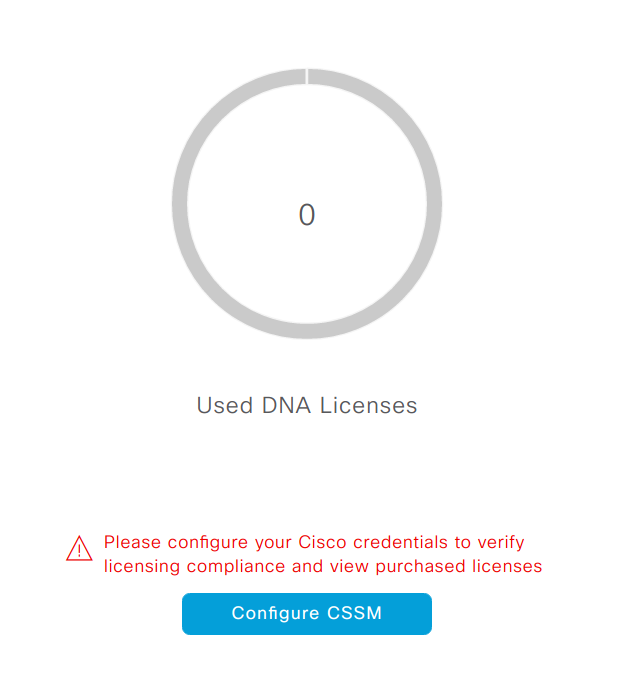
\includegraphics[height=6cm]{img/Selection_006.png}
	\caption{Ohne verlinkten CSSM Account können keine Lizenzen zugewiesen werden.}
	\label{fig:dna-center-licence-3}
\end{figure}

\begin{figure}[H]
	\centering
	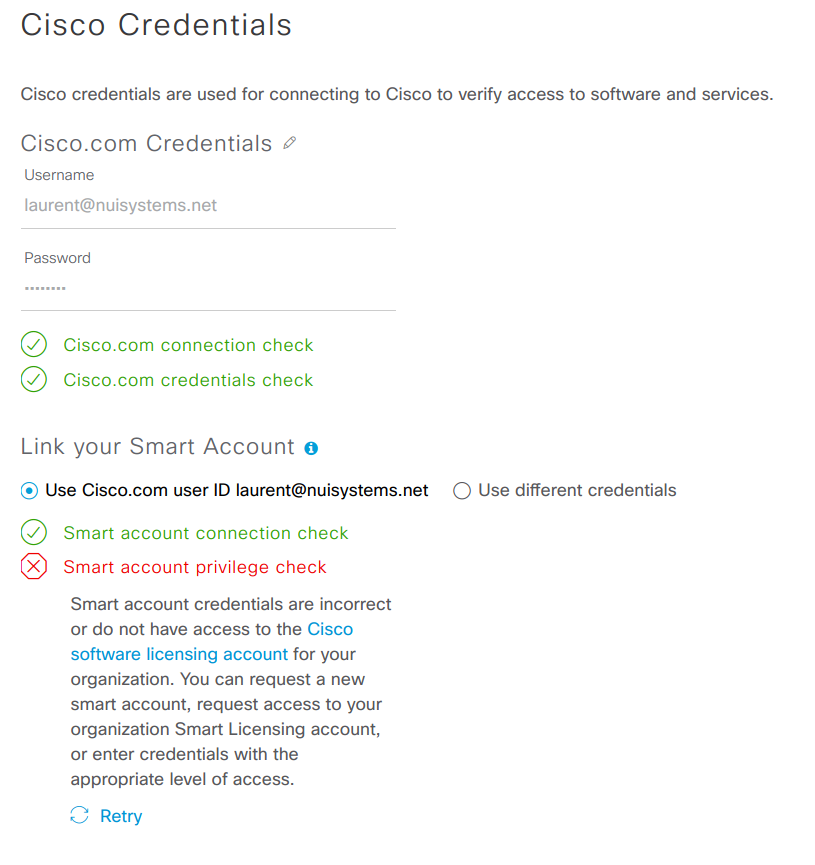
\includegraphics[height=6cm]{img/Selection_008.png}
	\caption{Der im DNA Center hinterlegte Cisco Account muss Zugriff zum entsprechenden Smart Account haben.}
	\label{fig:dna-center-licence-4}
\end{figure}

\begin{figure}[H]
	\centering
	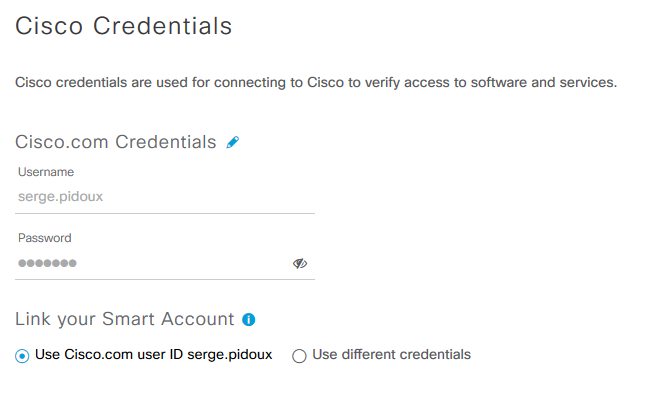
\includegraphics[height=5cm]{img/LicenceManager_002.png}
	\caption{Der korrekt hinterlegte Account}
	\label{fig:dna-center-licence-5}
\end{figure}

\begin{figure}[H]
	\centering
	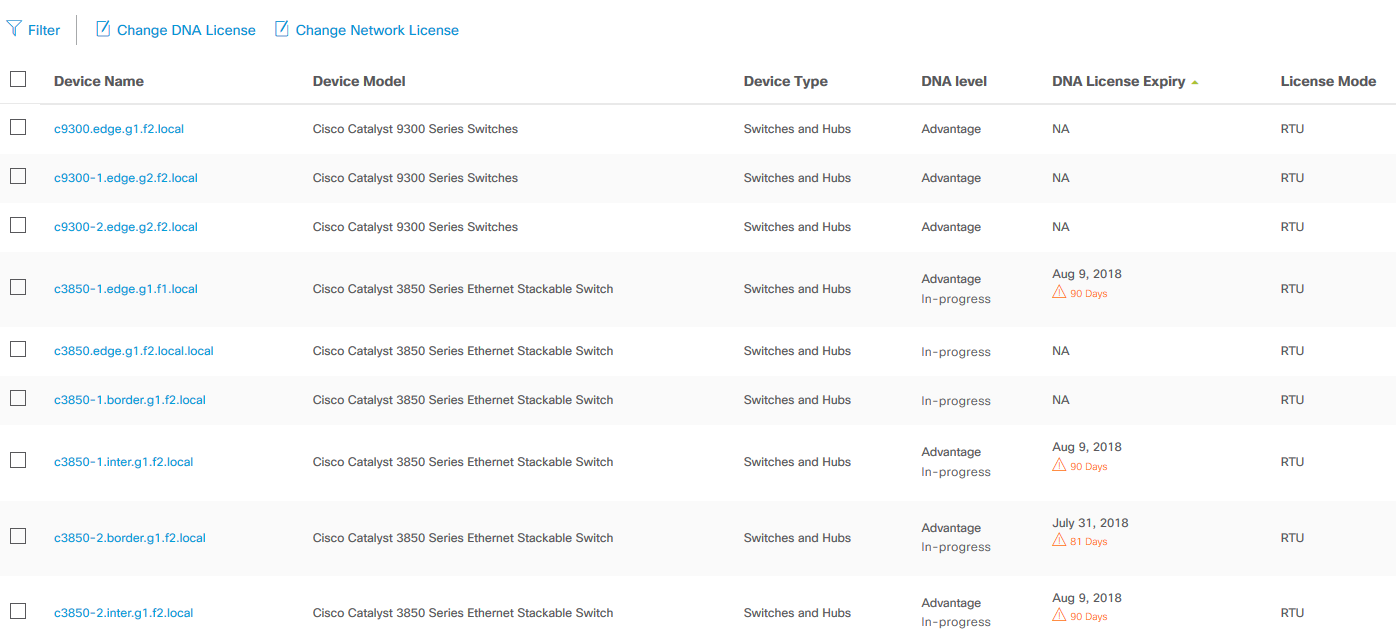
\includegraphics[height=8cm]{img/LicenceManager_003.png}
	\caption{Übersicht über die den Netzwerkkomponenten zugewiesenen Lizenzen}
	\label{fig:dna-center-licence-6}
\end{figure}

\begin{figure}[H]
	\centering
	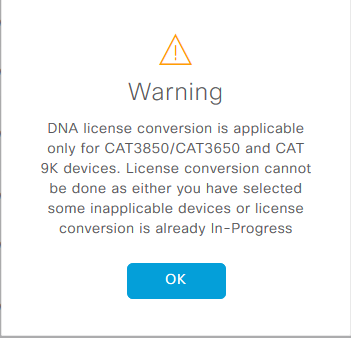
\includegraphics[height=6cm]{img/LicenceManager_004.png}
	\caption{Nicht jedem Gerät kann eine Lizenz zugewiesen werden (Siehe Tabelle)}
	\label{fig:dna-center-licence-7}
\end{figure}

\begin{tabular}{ | c | c | }
	\hline
	\textbf{Geräteserie} & 	\textbf{Lizenzzuweisung möglich} \\
	\hline
	Cisco Catalyst 9300 Series Switches & Ja \\
	\hline
	Cisco Catalyst 3850 Series Ethernet Stackable Switch & Ja \\
	\hline
	Cisco 4400 Series Integrated Services Routers & Nein \\
	\hline
\end{tabular}

\subsection{Device Provisioning via DNA Center}
Um den einzelnen Netzwerkgeräten einen Namen und die Basis Konfiguration zu geben, werden im DNA Center unter \textit{Provision $\rightarrow$ Devices} die zu provisionierenden Geräte ausgewählt. Danach wird \textit{Action $\rightarrow$ Provision Device} der Provision Vorgang gestartet.

Dabei wird die komplette Konfiguration, die das DNA Center für ein Device vorsieht auf dem Gerät konfiguriert. Sind Templates für den entsprechende Devicetyp konfiguriert worden, werden diese ebenfalls angewendet.
Templates können im Template Editor erstellt und entsprechenden Gerätetypen zugewiesen werden.

\begin{figure}[H]
	\centering
	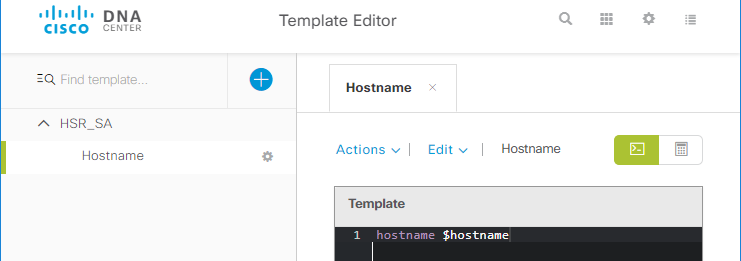
\includegraphics[width=12cm]{img/templateeditor.png}
	\caption{Template Editor}
	\label{fig:Template Editor}
\end{figure}


\subsection{Fabric Konfigurieren}
Nach der manuellen Konfiguration des Underlays, dem hinzufügen der Geräte, dem Update und dem Provisionieren, konnten wir endlich die Fabric konfigurieren. 

Erreichbar ist das unter \textit{Provision $\rightarrow$ Fabric}. Nachfolgend wird die Fabric des entsprechenden Standortes ausgewählt.

Den einzelnen Netzwerkgeräten werden nun mit Rechtsklick folgende Rollen zugeteilt:
\begin{itemize}
	\item Border
	\item Border + CP (Control Plane)
	\item Edge
\end{itemize}

Nachdem alle Geräte der entsprechenden Fabric zugeteilt worden sind, kann die Konfiguration gespeichert werden und wird auf die Geräte geschrieben. 

\begin{figure}[H]
	\centering
	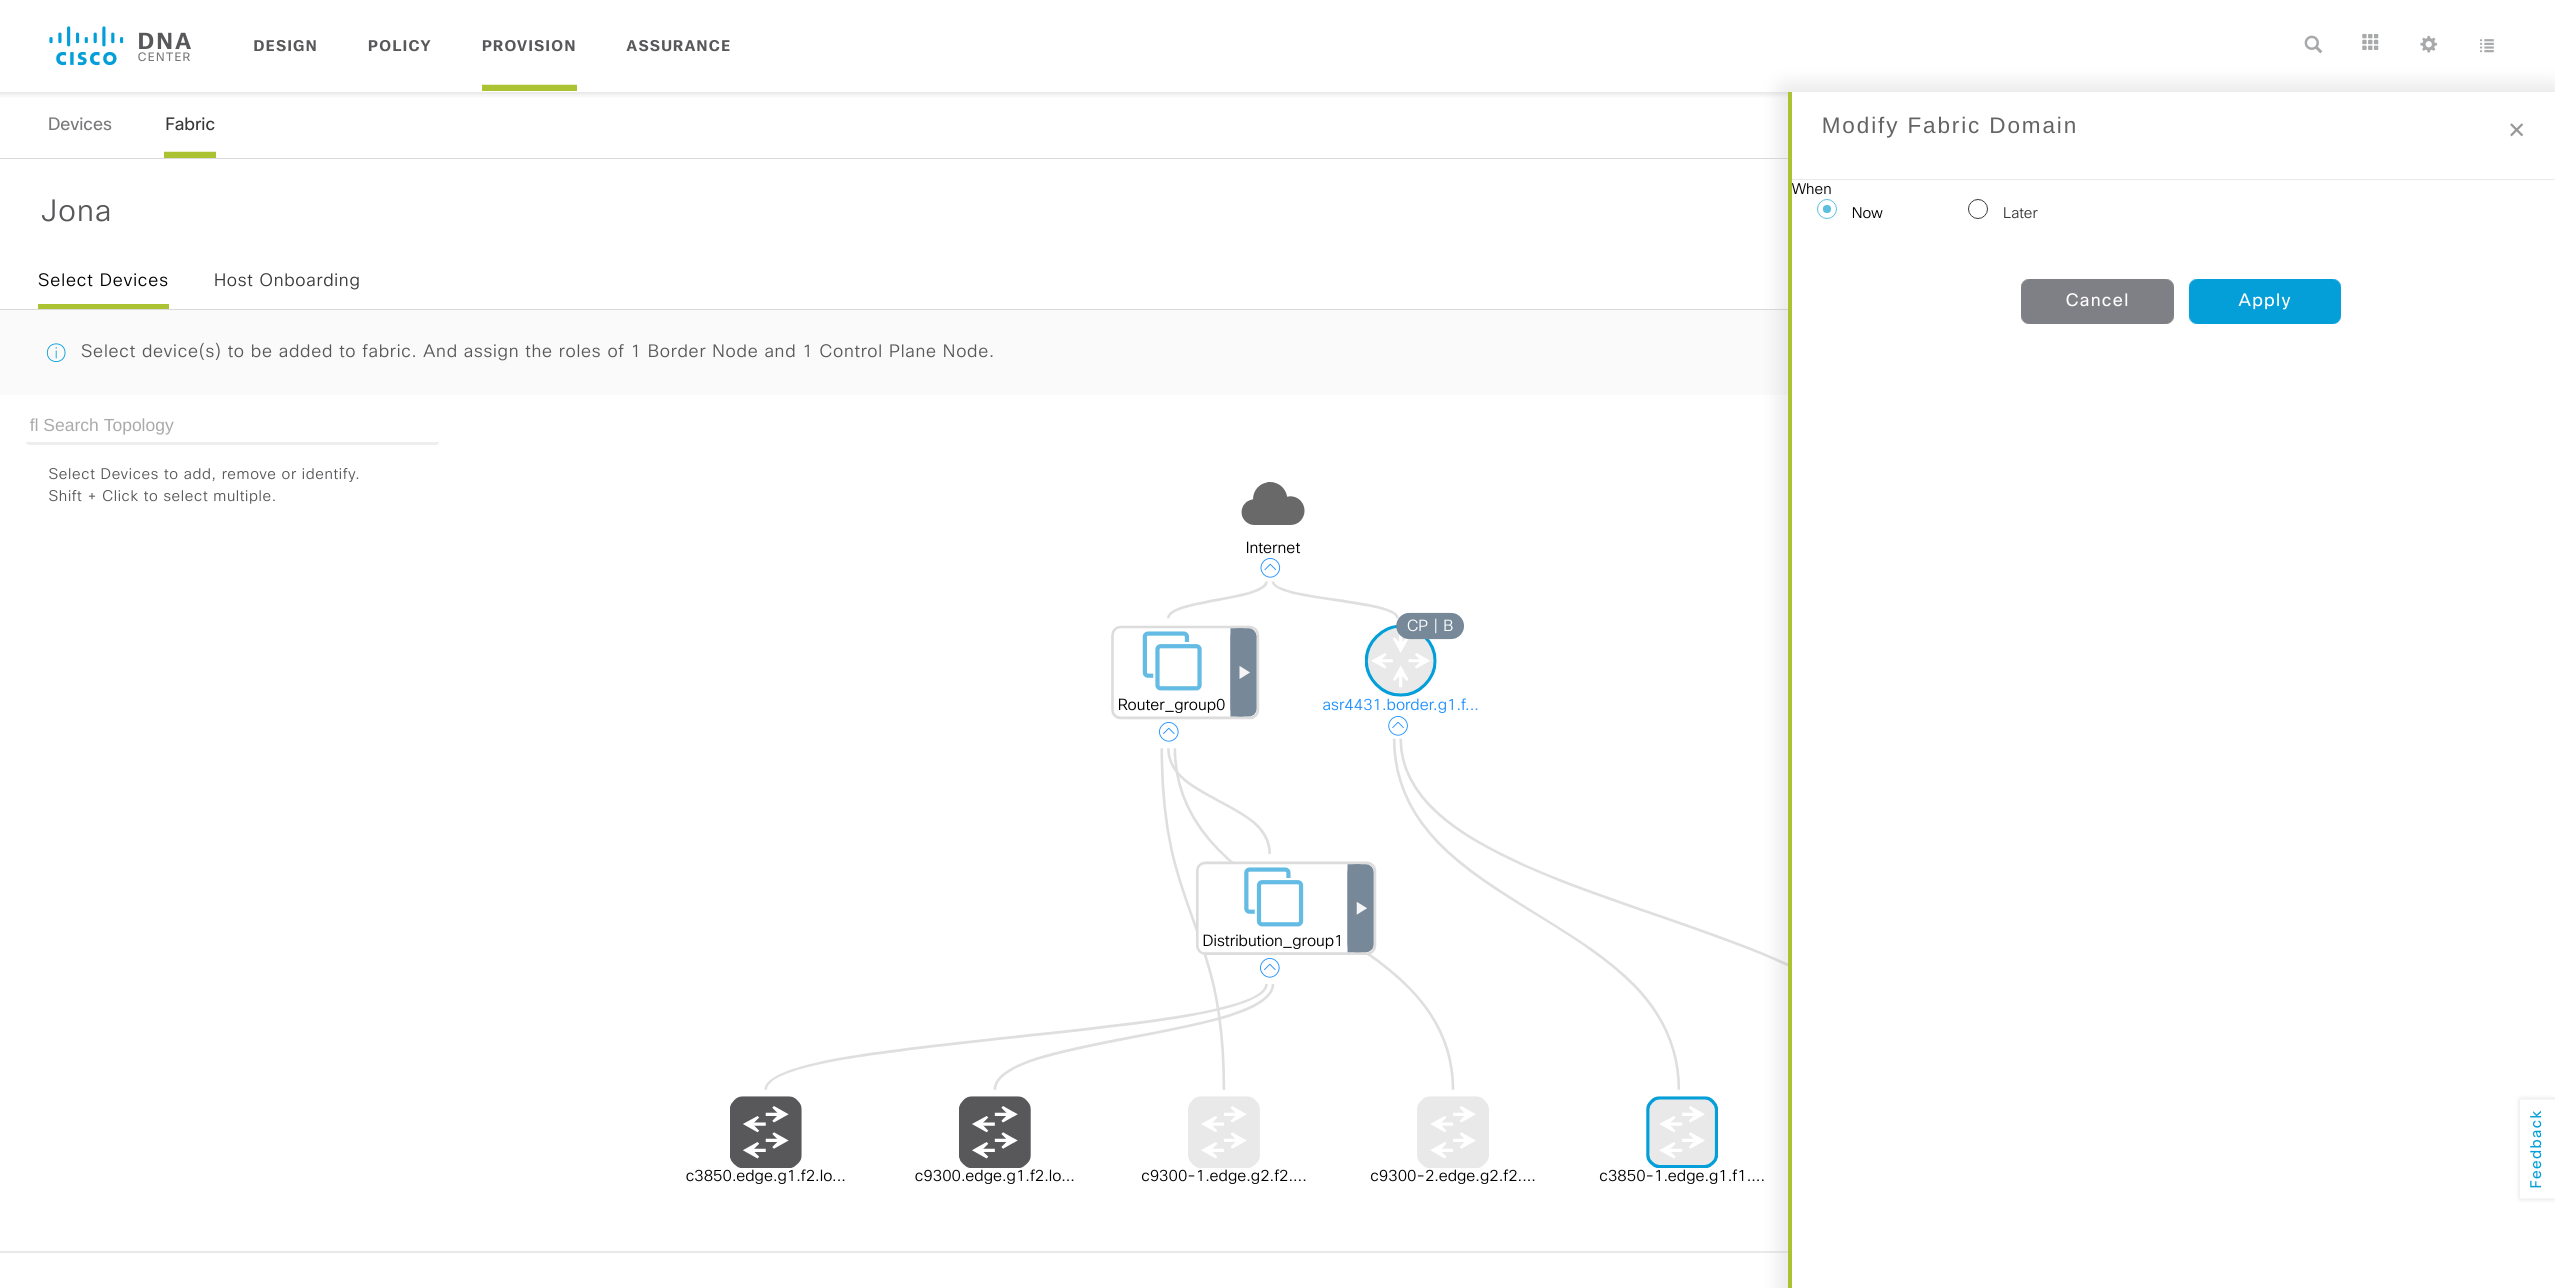
\includegraphics[width=16cm]{img/dna-center-fabric-1.png}
	\caption{DNA Center Provision - Fabric - Nach der Zuteilung wird die Konfiguration auf die Geräte geschrieben.}
	\label{fig:IP Base and Services}
\end{figure}


\begin{tabular}{| l | l | l | l | l |}
	\hline
	\textbf{Darstellung} & \makecell{\textbf{Teil der}\\ \textbf{Fabric}} & \makecell{\textbf{Änderung}\\ \textbf{ausstehend}} & \textbf{Provisioniert} & \textbf{Bemerkung} \\
	\hline
	Grau & Ja & Nein & Nein & \\
	Schwarz & Nein & Nein & Nein & \\
	Grau mit blauem Rand & Ja & Ja & Nein & \\
	Blau & Ja & Nein & Ja & \\
	Umrandung mit Pfeil & - & - & - & Gruppierte Geräte\\	
	\hline
\end{tabular}
\captionof{table}{DNA Center Provision - Fabric - Darstellung}


\subsection{DNA Center Reset}
Da das Overlay Provisioning auch nach mehreren Versuchen nur teilweise funktioniert hatte, haben wir entschlossen, die Switches zusätzlich über das Out-of-Band Management zu verbinden, da diese in mehreren Videos von Cisco so erwähnt wird und im ersten Release zwingend nötig war. \\
Dazu benötigt das DNA Center ein zusätzliches Interface im Out-of-Band Management Netz. Um dieses einzurichten, muss der initiale Wizard erneut gestartet werden. 

\begin{lstlisting}[language=bash]
$ maglev-config-wizard #DO NOT EXECUTE THIS COMMAND
\end{lstlisting}

Als folge dieses Befehls, nachdem alle Parameter eingegeben wurden, kam die folgende Meldung:

\begin{figure}[H]
	\centering
	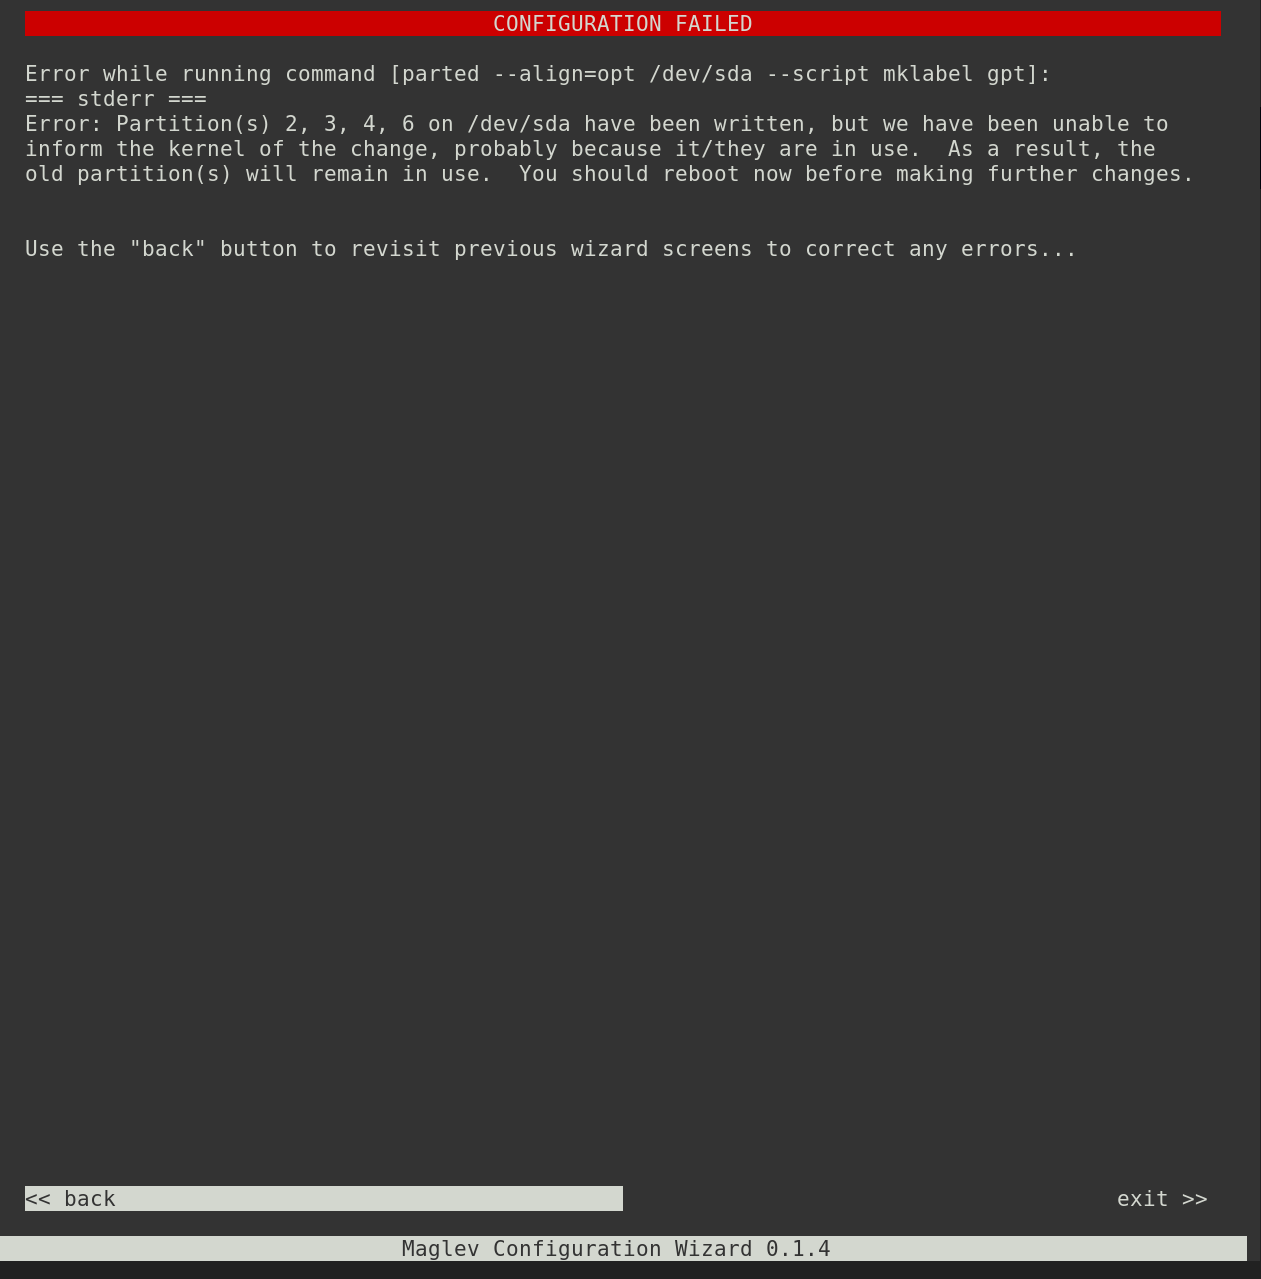
\includegraphics[height=10cm]{img/dna-center-reset-fail-1.png}
	\caption{DNA Center - maglev-config-wizard - Fehlermeldung}
	\label{fig:dna-center-reset-1}
\end{figure}

Nach einem Neustart der Appliance kam die folgende Meldung und das System bootete nicht mehr. 
\begin{figure}[H]
	\centering
	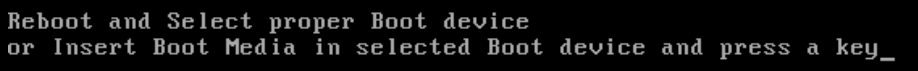
\includegraphics[height=1cm]{img/dna-center-reset-fail-2.png}
	\caption{DNA Center - Boot Fehlermeldung}
	\label{fig:dna-center-reset-2}
\end{figure}

Korrekt wäre der folgende Befehl gewesen:

\begin{lstlisting}[language=bash]
$ sudo maglev-config update
\end{lstlisting}

Allerdings hätte auch der erste Befehl nicht dazu führen sollen, dass das System nicht mehr startet.

\paragraph{Neuinstallation}\\
In der Folge war es nötig, dass DNA Center komplett neu zu installieren. Dazu ist ein entsprechendes ISO nötig, welches leider nicht mitgeliefert wird. Dieses kann bei Cisco via TAC Case angefordert werden. Mit dem ISO muss dann ein bootbarer USB Stick erstellt werden.

\begin{figure}[H]
	\centering
	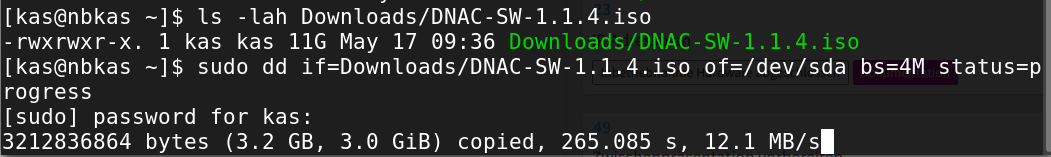
\includegraphics[height=2cm]{img/dna-center-reset-iso.png}
	\caption{DNA Center - Neuinstallation - Installations ISO wird auf USB Drive kopiert}
	\label{fig:dna-center-iso-1}
\end{figure}

Anschliessend kann der USB-Stick in die Appliance gesteckt und diese gestartet werden. Die initiale Installation ist in Abschnitt \ref{DNACenterSetup_Installation} gezeigt. 

\alertwarningbox{
	Nach der Neuinstallation sind alle Daten und die Konfiguration gelöscht. Eine Option die Konfiguration beizubehalten gibt es nicht.
}

\section{Vorgehen Versuch 2}

\subsection{DNA Center Netzwerk Design}
Wie im ersten Teil

\subsection{Downgrade aller Netzwerkkomponenten}
Nach Absprache mit dem Experten von Cisco, mussten alle Switch und Router auf eine spezifische Version zurückgesetzt werden.

Neue Version: 16.6.3

\subsection{ISE reset}
Um die Störungen durch alte Konfigurationen zu vermeiden, wurde das Cisco ISE Center ebenfalls zurückgesetzt. Dies kann einfach mittels eines Befehls durchgeführt werden.

\begin{lstlisting}[language=bash]
ISE/admin# applicaiton reset-config ise
\end{lstlisting}

\begin{figure}[H]
	\centering
	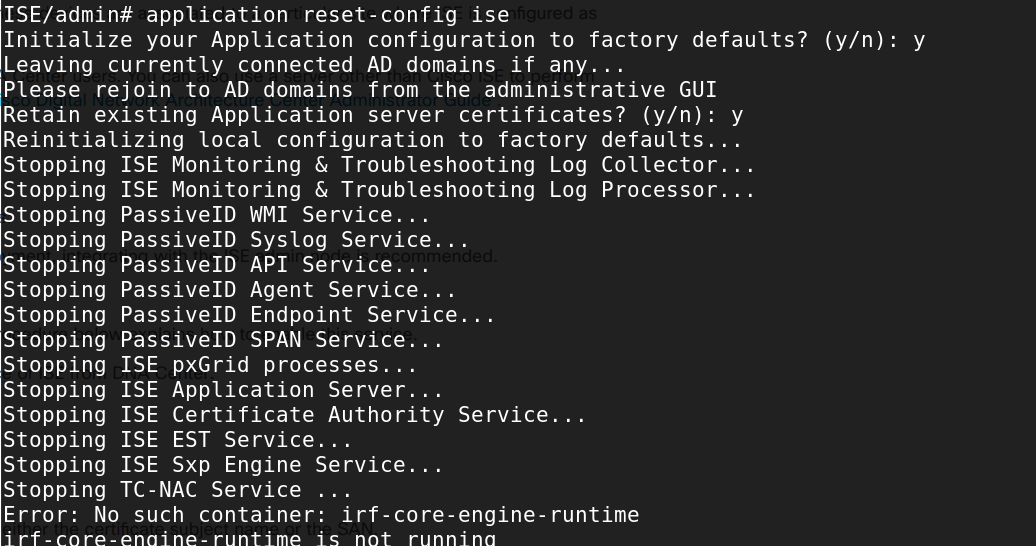
\includegraphics[height=6cm]{img/secondtry/s2t-cisco-ise-reset.png}
	\caption{Cisco ISE Reset}
	\label{fig:dna-ise-reset-1}
\end{figure}

\subsection{Credentials korrekt hinterlegen}
TBA

\subsection{ISE Integration}
TBA

\subsection{Fabric Border - Seeddevice}
Bevor die LAN Automation gestartet werden kann, müssen folgende Bedinungen erfüllt sein:
\begin{itemize}
	\item Aktives SSH
	\item IP Konnektivität
\end{itemize}

\subsubsection{Verbindung zwischen Legacy Router und Border Switch}
Um eine Verbindung über den Legacy Router zu ermöglichen, musste ein VLAN angelegt werden.

\paragraph{Konfiguration auf Border Switch}
\begin{lstlisting}[language=bash]
# interace XY
# switchport trunk native vlan 100
# interface vlan 100
# ip adress 10.22.31.1 255.255.255.252
# exit
# ip route 10.22.0.0 255.255.255.0 10.22.31.0
\end{lstlisting}

\paragraph{Konfiguration auf Legacy Router}
\begin{lstlisting}[language=bash]
# interface GigabitEthernet0/0/1.100
# encapsulation dot1Q 100
# ip address 10.22.31.2 255.255.255.252
\end{lstlisting}

\subsection{Border BGP}
\begin{lstlisting}[language=bash]
router bgp 10
bgp log-neighbor-changes
neighbor 10.22.11.1 remote-as 30
address-family ipv4
redistribute connected
neighbor 10.22.11.1 activate
exit-address-family
\end{lstlisting}

\subsection{Trustpool}
Zuvor ist das Zertifikat des DNA Centers ersetzt worden. Den gemäss \cite{cisco-dna-appliance-installation-guide-release-1-1} ist es für den ISE Version 2.4 erforderlich, dass die IP Adresse des DNA Centers im Zertifikat hinterlegt worden. Da die Version 2.4 sowieso nicht mit dem DNA Center Version 1.1.5 kompatibel ist, musste der ISE in der Version 2.3 neu installiert werden. Dies hat diese spezielle Anforderung an das Zertifikat nicht. Da das benutzerdefinierte Zertifikat die LAN Automation behinderte. Stellten wir das alte Zertifikat wieder her.

Mit dem folgenden Befehl konnte das ursprüngliche Zertifikat lokal heruntergeladen.

\begin{lstlisting}[language=bash]
scp -r -P 2222 maglev@10.22.0.100:/etc/maglev/.pki .
\end{lstlisting}

In DNA Center unter \textit{System Settings $\rightarrow$ Settings $\rightarrow$ Certificate} wurde das gebergte Zertifikat eingespielt. 

\begin{figure}[H]
	\centering
	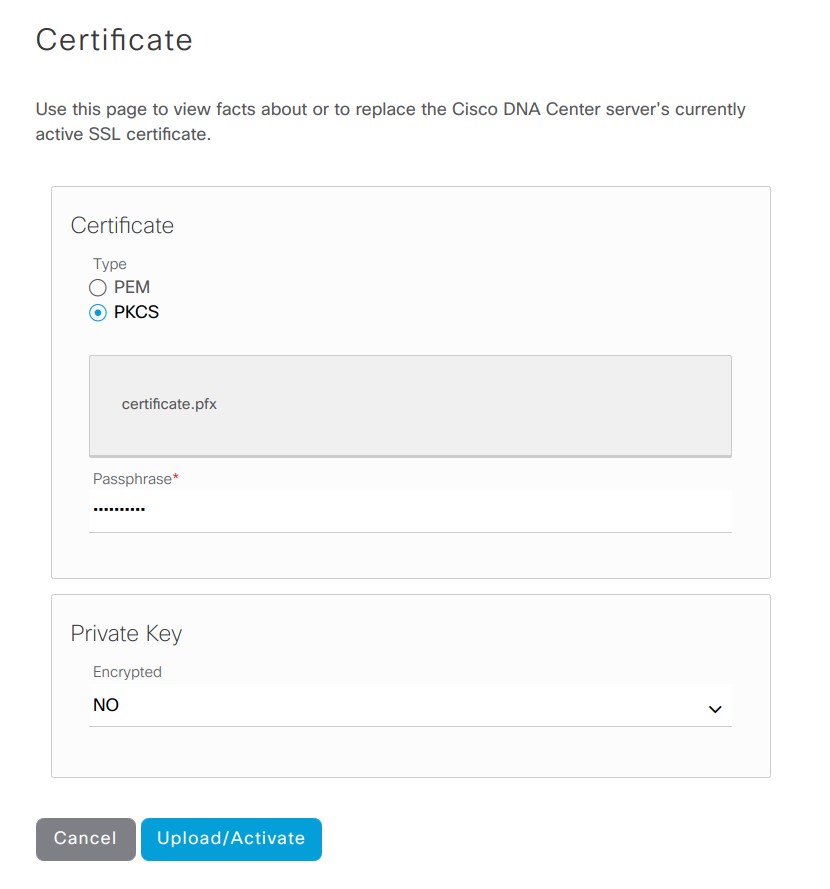
\includegraphics[height=8cm]{img/secondtry/dna-center-replace-certificate.png}
	\caption{Cisco DNA Center - Zertifikat ändern}
	\label{fig:dna-zertificate-1}
\end{figure}


\subsection{Netzwork Discovery - LAN Automation - Zweiter Versuch}
\label{Netzwork Discovery - LAN Automation - Zweiter Versuch}
Die Netzwerk Discovery braucht mehr Eingriffe als erwartet. Im ersten Schritt haben wir versucht alle Geräte auf der Seite Rapperswil einzuspielen. Dies hat nicht geklappt. Das PNP schlägt fehl. Deshalb sind wir wie folgt vorgegangen:
\begin{enumerate}
	\item Ein Netzwerkgerät im \textit{Initial Config Dialog} Zustand lassen. (Siehe: \ref{fig:cisco-switch-initial-config})
	\item LAN Automation durchführen. (Siehe \ref{fig:dna-lan-automation-dialog})
	\item Vorgang wiederholen, bis alle Geräte hinzugefügt sind. 
\end{enumerate}

\begin{figure}[H]
	\centering
	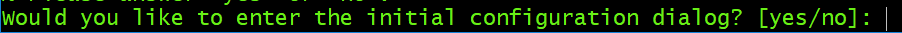
\includegraphics[height=0.5cm]{img/secondtry/cisco-switch-initial-config.png}
	\caption{Cisco Switch - Initial Config - Versucht DHCP und PNP zu machen, solange der Dialog aktiv ist.}
	\label{fig:cisco-switch-initial-config}
\end{figure}

\begin{figure}[H]
	\centering
	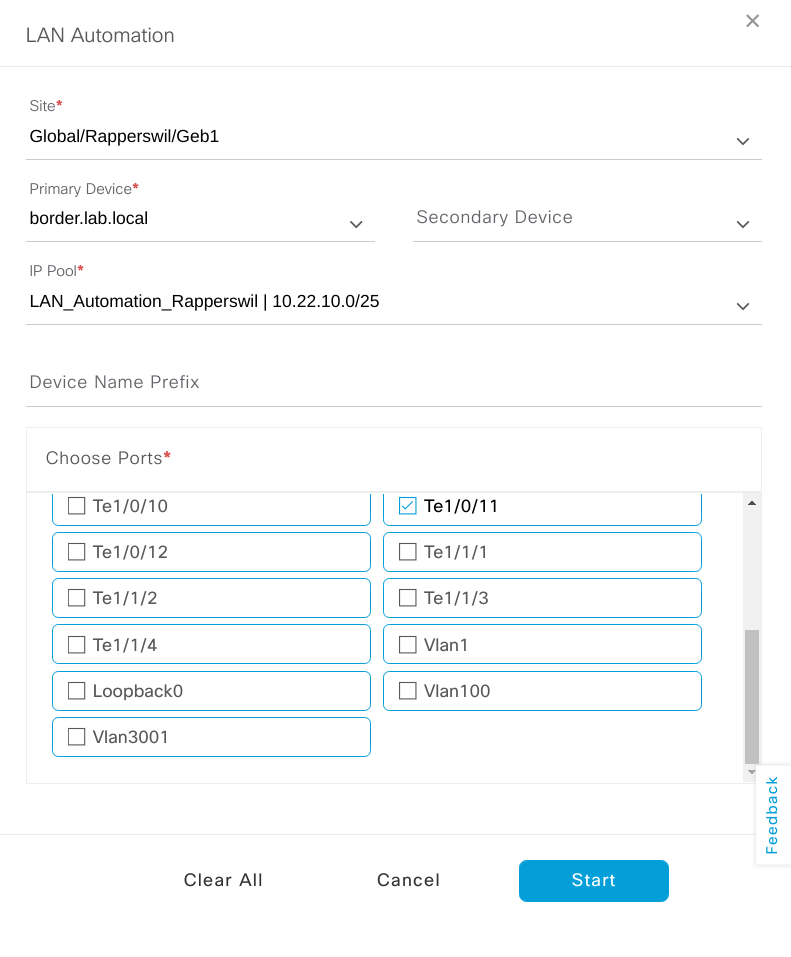
\includegraphics[height=7cm]{img/secondtry/dna-lan-automation-dialog.png}
	\caption{Cisco Switch - DNA LAN Automation}
	\label{fig:dna-lan-automation-dialog}
\end{figure}

\alertwarningbox{
	Die LAN Automation funktionierte nur mit den Standard Zertifikaten. 
}

\subsection{Broken ISIS - Gründe}
TBA

\subsection{Provisioning}

\subsubsection{Script Template}
\label{Script Template}
Damit der Hostname der Switches und Router via Provisioning gesetzt werden kann, muss ein Template angelegt werden.

Über das Hauptmenü \textit{Tools $\rightarrow$ Template Editor} kann mit \textit{Add (Pluszeichen) $\rightarrow$ Create Project} ein neues Projekt anlegt werden. (Siehe: \ref{fig:dna-center-template-editor-add-project})

\begin{figure}[H]
	\centering
	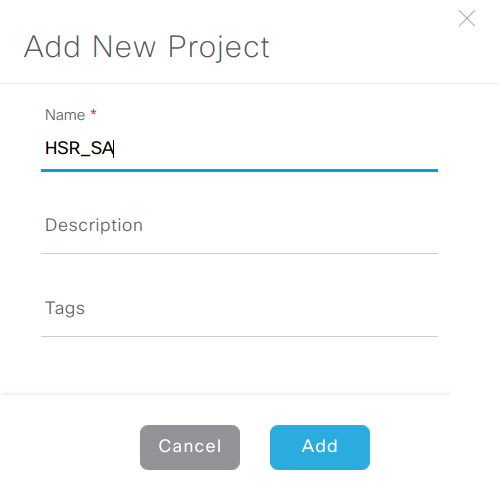
\includegraphics[height=7cm]{img/secondtry/dna-center-template-editor-add-project.png}
	\caption{Cisco DNA Center - Templateeditor - Add Project}
	\label{fig:dna-center-template-editor-add-project}
\end{figure}

Weiter kann mit \textit{Add (Pluszeichen) $\rightarrow$ Add Template} ein neues leeres File angelegt werden. (Siehe \ref{fig:dna-center-template-editor-add-template})

\begin{figure}[H]
	\centering
	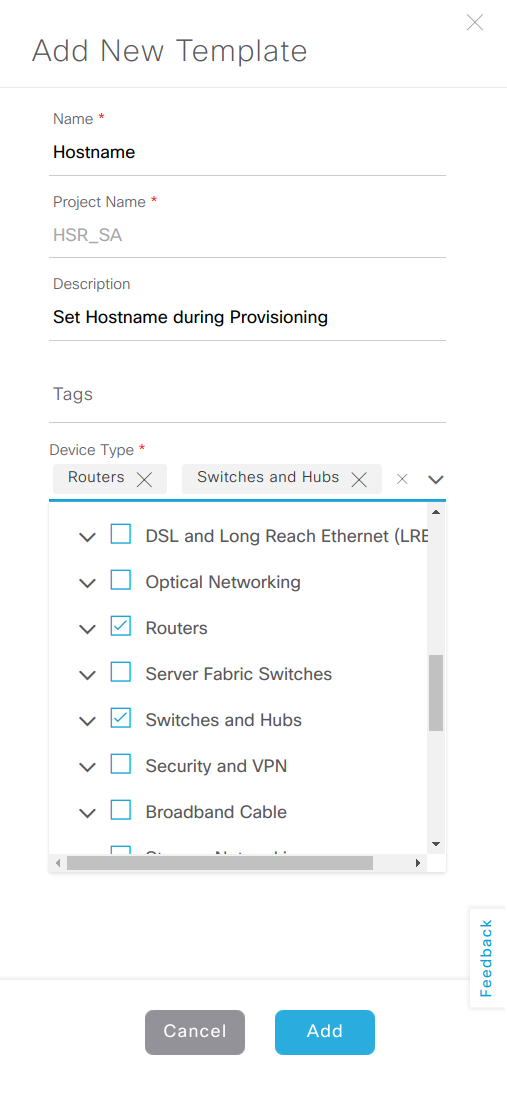
\includegraphics[height=7cm]{img/secondtry/dna-center-template-editor-add-template.png}
	\caption{Cisco DNA Center - Templateeditor - Add Template}
	\label{fig:dna-center-template-editor-add-template}
\end{figure}

Wie in Abbilung \ref{fig:dna-center-template-editor-add-template} sind folgende Einstellungen festzulegen:
\begin{itemize}
	\item Name des Templates
	\item Zugehörige Projekt
	\item Beschreinbung
	\item Tags
	\item Für welche \textit{Device Types} das Template verwendet werden soll.
\end{itemize}

\begin{figure}[H]
	\centering
	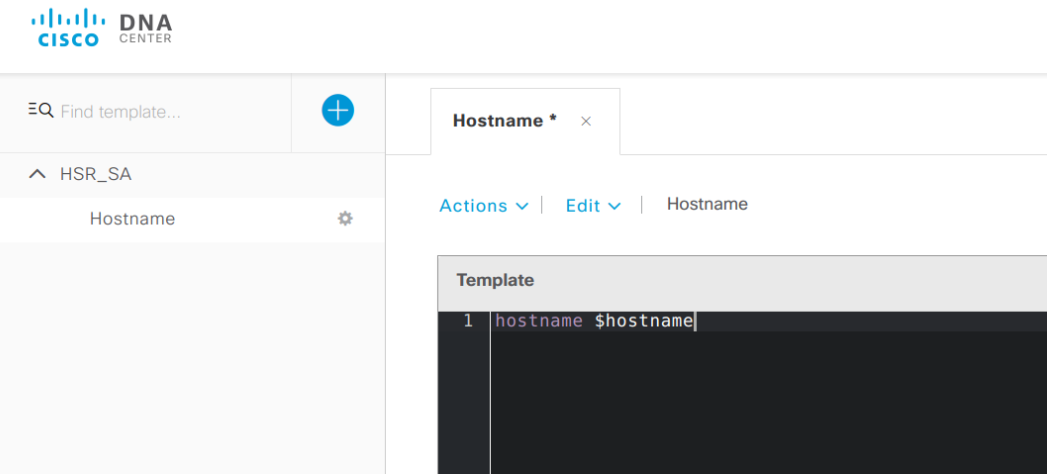
\includegraphics[height=7cm]{img/secondtry/dna-center-template-editor-edit.png}
	\caption{Cisco DNA Center - Templateeditor - Template um den Hostname bei der Provisionierung zu setzen.}
	\label{fig:dna-center-template-editor-edit}
\end{figure}

\subsubsection{Network Profile anlegen}
Unter \textit{Design $\rightarrow$ Network Profiles $\rightarrow$ Add Profile} kann ein neues Profil angelegt werden. Dieses Profil wird während des Provisionierungsvorgang verwendet. 

\begin{figure}[H]
	\centering
	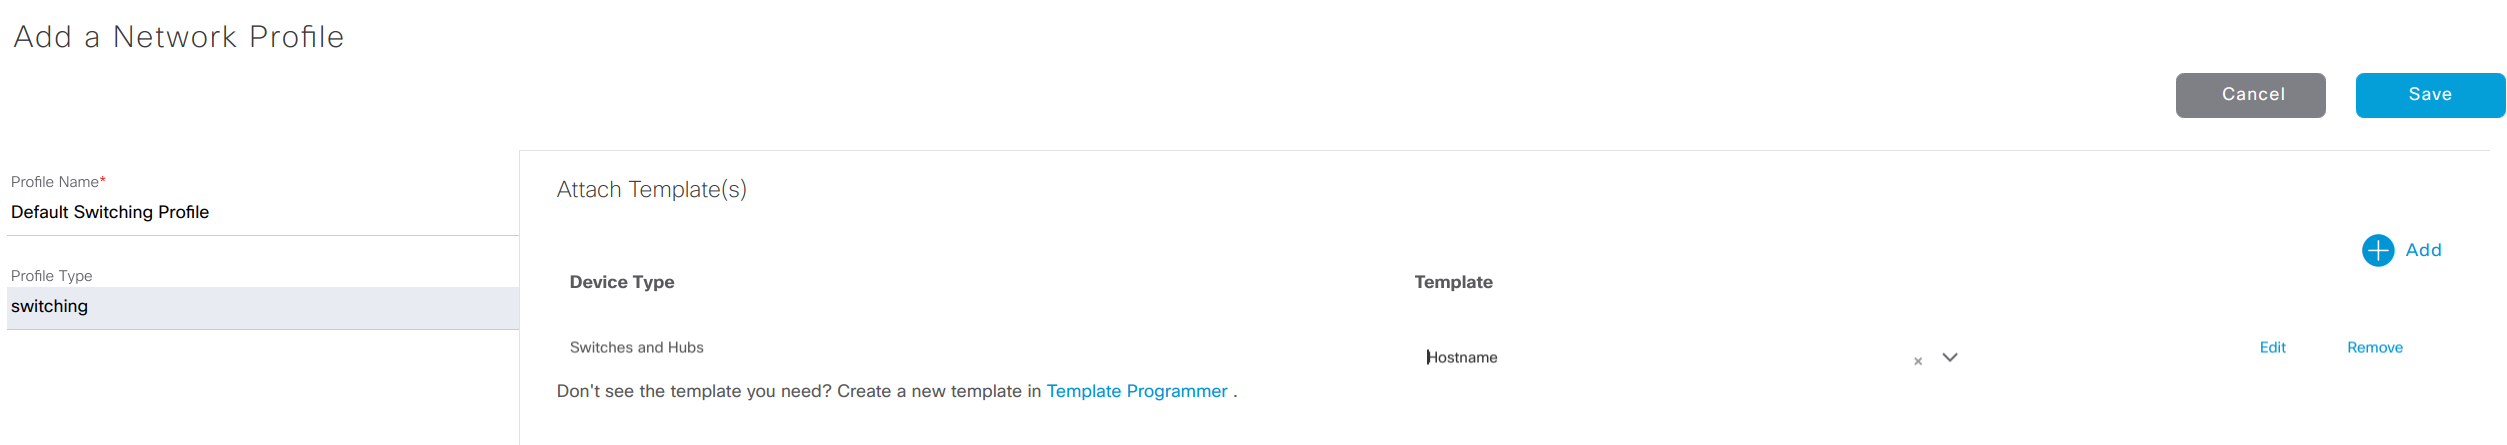
\includegraphics[height=4cm]{img/secondtry/dna-center-network-profile-new.png}
	\caption{Cisco DNA Center - Network Profile - New Profile}
	\label{fig:dna-center-network-profile-new}
\end{figure}

Weiter wird festgelegt für welche \textit{Sites} das Netzwerkprofil verwendet werden soll. 

\begin{figure}[H]
	\centering
	\includegraphics[height=5cm]{img/secondtry/dna-center-network-profile-assign-sites.png}
	\caption{Cisco DNA Center - Network Profile - Assign Sites}
	\label{fig:dna-center-network-profile-assign-sites}
\end{figure}

\subsubsection{Claimed Netzwerkgeräte Provisionierung}

Die Provisionierung gestaltet sich im Normalfall sehr einfach. Im Modul \textit{Provision $\rightarrow$ Devices $\rightarrow$ Inventory}

Das zu provisionierende Gerät wird in der Liste ausgewählt. Über \textit{Action $\rightarrow$ Provision} wird die Provision gestartet. 

\begin{figure}[H]
	\centering
	\includegraphics[height=5cm]{img/secondtry/dna-center-provision-device.png}
	\caption{Cisco DNA Center - Netzwerkgerät konfigurieren}
	\label{fig:dna-center-provision-device}
\end{figure}

Im ersten Schritt (Siehe: \ref{fig:dna-center-provision-step1}) wird die entsprechende \textit{Site} ausgewählt. 

\begin{figure}[H]
	\centering
	\includegraphics[height=3cm]{img/secondtry/dna-center-provision-step1.png}
	\caption{Cisco DNA Center - Provision Step 1}
	\label{fig:dna-center-provision-step1}
\end{figure}

Im zweiten Schritt gibt es keine wählbaren Optionen. 

Im dritten Schritt kann das in im Abschnitt \cite{Script Template} ausgewählt werden. Die offnen Variablen (im Falle \ref{fig:dna-center-provision-step3}) werden hier hinterlegt. 

\begin{figure}[H]
	\centering
	\includegraphics[height=4cm]{img/secondtry/dna-center-provision-step3.png}
	\caption{Cisco DNA Center - Provision Step 3}
	\label{fig:dna-center-provision-step3}
\end{figure}

Im letzte Schritt erscheint eine Übersicht. Mit einem Klick auf \textit{Deploy} wird der Script provisioniert. Die dabei automatisch ausgeführten Befehle durch das DNA Center sind in Listing \ref{lst:commands-executed-during-provision} ersichtlich.


\begin{lstlisting}[caption={Befehle automatisch ausgeführt durch das DNA Center während der Provisionierung},label={lst:commands-executed-during-provision},language=bash]
enable
no ip domain-lookup 
ip access-list extended ACL_WEBAUTH_REDIRECT
180 permit tcp any any eq www 
190 permit tcp any any eq 443 
200 permit tcp any any eq 8443 
210 permit udp any any eq domain 
220 permit udp any eq bootpc  any eq bootps 
170 deny ip any host 10.22.0.22
exit 
ip tacacs source-interface Loopback0 
ip radius source-interface Loopback0 
aaa new-model 
ip radius source-interface Loopback 0
exit 
aaa group server radius dnac-network-radius-group
server name dnac-radius_10.22.0.22
ip radius source-interface Loopback 0
exit 
aaa accounting dot1x default start-stop group dnac-client-radius-group
aaa accounting update newinfo periodic 600
aaa accounting exec default start-stop group dnac-network-radius-group
aaa authorization network dnac-cts-list group dnac-client-radius-group
aaa authorization exec VTY_author group dnac-network-radius-group local if-authenticated 
aaa authorization exec VTY_author group dnac-network-radius-group local 
aaa authentication login default local 
aaa authentication dot1x default group dnac-client-radius-group
aaa authentication login VTY_authen group dnac-network-radius-group local 
dot1x system-auth-control 
radius server dnac-radius_10.22.0.22
address ipv4 10.22.0.22 auth-port 1812 acct-port 1813
pac key *
retransmit 1
radius-server deadtime 30
radius-server attribute 25 access-request include 
radius-server attribute 8 include-in-access-req 
radius-server attribute 6 on-for-login-auth 
radius-server attribute 6 support-multiple 
cts authorization list dnac-cts-list
line vty 0 97
login authentication VTY_authen
authorization exec VTY_author
transport input all 
enable
enable
banner motd #\"Welcome to our SA Lab!\"#
hostname c9300-2.edge.g2.f2
enable
enable
enable
enable
enable
enable
enable
\end{lstlisting}

\subsection{Fabric}

\subsubsection{Device Role zuordnen}

\subsubsection{Add to Fabric}
Screenshots und vorgehen. 

\begin{lstlisting}[caption={Befehle automatisch ausgeführt durch das DNA Center während dem hinzufügen zur Fabric},label={lst:commands-executed-during-add-to-fabric},language=bash]
!exec: enable
ip dhcp snooping 
cts role-based enforcement 
vrf definition DEFAULT_VN
address-family ipv4 
vlan 4000
name VOICE_VLAN
exit 
vlan 3999
name CRITICAL_VLAN
exit 
interface GigabitEthernet1/0/3 
no load-interval 
no spanning-tree portfast 
no switchport trunk native vlan 
switchport 
switchport mode dynamic auto 
switchport access vlan 1
exit 
interface GigabitEthernet1/0/4 
no load-interval 
no switchport trunk native vlan 
switchport 
switchport mode dynamic auto 
switchport access vlan 1
exit 
interface GigabitEthernet1/0/7 
no load-interval 
no spanning-tree portfast 
no switchport trunk native vlan 
switchport 
no switchport trunk native vlan 
switchport 
switchport mode dynamic auto 
switchport access vlan 1
exit 
interface GigabitEthernet1/0/10 
no load-interval 
no spanning-tree portfast 
no switchport trunk native vlan 
switchport 
interface GigabitEthernet1/0/12 
no load-interval 
no spanning-tree portfast 
no switchport trunk native vlan 
switchport 
switchport mode dynamic auto 
switchport access vlan 1
exit 
interface GigabitEthernet1/0/13 
no load-interval 
no switchport trunk native vlan 
switchport 
switchport mode dynamic auto 
switchport access vlan 1
exit 
interface GigabitEthernet1/0/15 
no load-interval 
no spanning-tree portfast 
no switchport trunk native vlan 
switchport 
switchport 
switchport mode dynamic auto 
switchport access vlan 1
exit 
interface GigabitEthernet1/0/18 
no load-interval 
no spanning-tree portfast 
no switchport trunk native vlan 
switchport 
switchport mode dynamic auto 
switchport access vlan 1
exit 
interface GigabitEthernet1/0/21 
no load-interval 
no spanning-tree portfast 
no switchport trunk native vlan 
switchport 
switchport mode dynamic auto 
switchport access vlan 1
exit 
switchport access vlan 1
exit 
router lisp 
ipv4 source-locator Loopback0 
locator-set rloc_def9f1a7-9572-4e74-afaf-44215f0fbbde
IPv4-interface Loopback0 priority 10 weight 10
exit 
locator-table default 
locator default-set rloc_def9f1a7-9572-4e74-afaf-44215f0fbbde
service ipv4 
etr map-server 10.22.10.67 proxy-reply 
etr 
sgt 
use-petr 10.22.10.67
use-petr 10.22.30.1
exit 
service ethernet 
database-mapping limit dynamic 5000
map-cache-limit 25000
itr map-resolver 10.22.30.1
ipv4 locator reachability exclude-default 
ip dhcp relay information option 
banner motd #\"Welcome to our SA Lab!\"#
ip sla 1
icmp-echo 10.22.0.22 source-ip 10.22.10.65
frequency 60
threshold 3
timeout 5000
ip sla schedule 1  life forever start-time now 
banner motd #\"Welcome to our SA Lab!\"#
ip sla 2
icmp-echo 10.22.10.67 source-ip 10.22.10.65
frequency 60
threshold 3
timeout 5000
ip sla schedule 2  life forever start-time now 
banner motd #\"Welcome to our SA Lab!\"#
ip sla 3
icmp-echo 10.22.30.1 source-ip 10.22.10.65
frequency 60
threshold 3
timeout 5000
ip sla schedule 3  life forever start-time now 
banner motd #\"Welcome to our SA Lab!\"#
\end{lstlisting}

\subsection{LAN Automation - Dritter Versuch}
Da das DNA Center nur ein Teil der Links zwischen den Switches konfiguriert hat, entschieden wir uns diese nochmals neu durchzuführen. Ausser dem Seed Device haben wir alle Devices gelöscht. Danach starteten wir die LAN Automation nochmals (siehe Abschnitt \ref{Netzwork Discovery - LAN Automation - Zweiter Versuch}).

\begin{enumerate}
	\item LAN Automation starten
	\item Switches und Router so lange neu Booten bis PNP erfolgreich ist.
	\item LAN Automation stoppen
\end{enumerate}

\paragraph{Resultat}
Alle Devices und Links wurden erfolgreich konfiguriert. Das "Schritt-für-Schritt" hinzufügen vom vorherigen Versuch funktioniert nicht. Möglicherweise ist das spätere automatische Hinzufügen von Netzwerkgeräten zu einem Underlay nicht möglich. 

\subsection{Lizenzen auf Netzwerkgeräten nach Underlay Automation}
Geräte haben nicht mer EVAL sondern plötzlich Permanent Lizenzen

\subsection{Ping to Clients}

\subsection{Host Onboarding}

Infoblox vorgehen bei neuem Netzwerk!!!

\subsubsection{Authentifizierungsmethoden}

\begin{tabular}{ | m{8cm} | m{8cm} | }
	\hline
	\textbf{Typ} & 	\textbf{Beschreibung} \\
	\hline
	Closed Authentication & Based on 802.1X. Authentication MUST succeed prior to network access. Requires networks with complete 802.1x support. \\
	Open Authentication & Based on 802.1x. Temporary access is granted (e.g. PXE, DHCP) prior to authentication. Optimal for networks with limited 802.1x support. \\
	Easy Connect & Based on LDAP combined with MAC Address Bypass (MAB). Optimal for networks using Active Directory (AD) authentication. \\
	No Authentication & Optimal for networks that do not support authentication or require static configuration. \\
	\hline

\end{tabular}
\caption[Erklärung der Host Onboardning Authentifizierungsmethoden]{Erklärung der Host Onboardning Authentifizierungsmethoden.\cite{ivan-caduff-slack}}

